\documentclass{vldb}
%\usepackage{times}

% do not change these values
%\baselineskip 12pt
%\textheight 10in
\textheight 674pt
%\textwidth 6.9in
%\oddsidemargin -0.3in
%\topmargin -0.3in
%\headheight 0in
%\headsep 0in

%\usepackage[utf8]{inputenc}
%\usepackage[english]{babel}

\usepackage{amsfonts}
\usepackage{graphicx}
\usepackage{balance}  % for  \balance command ON LAST PAGE  (only there!)
\usepackage[caption=false,font=footnotesize]{subfig}
\usepackage{amsmath}
\usepackage{amsopn}
\usepackage{comment}
\usepackage[ruled,linesnumbered]{algorithm2e}
\usepackage{multirow}
\usepackage{enumitem}

\begin{document}

\newcommand{\Paragraph}[1]{\smallskip{\bf #1.}}
\newcommand{\Paragraphnopunc}[1]{\smallskip\noindent{\bf #1}}
\newcommand{\Paragraphwithindent}[1]{\smallskip{\bf #1.}}
\newcommand{\tabincell}[2]{\begin{tabular}{@{}#1@{}}#2\end{tabular}}
\newcommand{\argmin}{\text{arg}\,\text{min}}
\newcommand{\argmax}{\text{arg}\,\text{max}}

%\theoremstyle{definition}
\newtheorem{definition}{Definition}
\newtheorem{prop}{Proposition}
\newtheorem{lemma}{Lemma}
\newtheorem{theorem}{Theorem}


\title{LayerLSH: Rebuilding Locality-Sensitive Hashing Indices by Exploring Density of Hash Values}
\author{
\alignauthor
Yanfeng Zhang, Xun Wei, Ge Yu\\
      \affaddr{Northeast University, China}\\
       \email{\{zhangyf, yuge\}@mail.neu.edu.cn, 1670851@stu.neu.edu.cn}
}
\date{}
\maketitle

\begin{abstract}
Locality-sensitive hashing (LSH) is known as one of the most promising indexing methods for approximate nearest neighbors (NN) search. It has attracted extensive research efforts for improving search quality. Many LSH variants are proposed in recent years. However, most of these LSH-based index structures fail to take data distribution into account. They perform well in a uniform data distribution setting but exhibit instable performance when the data are skewed. As known, most real life data are skewed, which makes LSH suffer. In this paper, we observe that the skewness of hash values resulted from skewed data is a potential reason for performance degradation. To address this problem, we propose to rebuild LSH indices by exploring the density of hash values. The hash values in dense ranges are reorganized with a multi-layered structure, so that more efforts are put into indexing the dense hash values. We rebuild three representative LSH indices for illustration, the table-based structure E2LSH, the tree-based structure LSB, and the recently proposed data sensitive hashing DSH. We further discuss the benefit in distributed computing. Extensive experiments are conducted to show the effectiveness and efficiency of the reconstructed LSH indices.
\end{abstract}


\IEEEraisesectionheading{\section{Introduction}\label{sec:intro}}

%The nearest neighbors (NN) search problem aims to find objects that are close to the given query, which is the basic and important problem in a wide range of applications, such as artificial intelligence, pattern recognition, information retrieval and so on. However, as the dimensionality of data objects increases, the performance of most existing methods \cite{kdtree,rtree,srtree} for exact NN search degenerates or be even worse than the brute-force linear-scan approach \cite{linscan}. Due to the difficulty in finding an efficient method for exact NN search in high-dimensional space, many researchers have focused on approximate nearest neighbors search as an alternative approach.

The nearest neighbors (NN) search problem aims to find objects that are close to the given query, which is the basic and important problem in a wide range of applications. Due to the difficulty in finding an efficient method for exact NN search in high-dimensional space, many researchers have focused on approximate nearest neighbors search as an alternative approach. Locality sensitive hashing (LSH) \cite{orilsh} is known as one of the most promising indexing methods for approximate nearest neighbors search, where the locality sensitive hash function has the property that points that are closer to each other have a higher probability of colliding than points that are farther apart. To improve the hashing effect, $m$ randomly chosen LSH functions are utilized together to generate a compound hash key for each object $o$. In compensation for the loss of candidate points because of importing compound hash key, a large number $l$ of hash tables are constructed.

\begin{comment}
\begin{Fig.}[t]
    \centerline{\includegraphics[width=2.8in]{fig/density_color.eps}}
    \caption{The distribution of point densities (KDD dataset).}
    \label{fig:density_query}
\end{Fig.}
\end{comment}


Many LSH variants have been proposed in recent years. From the index structure's point of view, these LSH variants can be classified into two categories, \emph{\textbf{table-based}} index \cite{Panigrahy:2006:EBN:1109557.1109688, mplsh,c2lsh,Haghani:2009:DSS:1516360.1516446,Huang:2015:QLH:2850469.2850470,Zheng:2016:LAN:2882903.2882930} and \emph{\textbf{tree-based}} index \cite{lsb,sklsh,Bawa:2005:LFS:1060745.1060840}. E2LSH \cite{datar} is a typical table-based LSH which proposes a hash function used in Euclidean space. The data points with the same hash value or the same concatenating hash values are placed in the same bucket, which implies that they are close to each other. The approximate NN search is achieved by returning the data in the same bucket as which the query falls in. Different from the intuitive table-based LSH structures, another set of LSH variants exploit tree structures. LSB \cite{lsb} and SK-LSH \cite{sklsh} share the similar idea that projects high-dimensional objects to a sequence of one-dimensional sortable values (e.g., $z$-value in LSB or compound hash key in SK-LSH), such that the linear order preserves the similarities between any two objects. The sequence of ordered values are then indexed by a B-tree like structure, and the NN search can be achieved by a bi-directional expansion process started from the B-tree node that corresponds to the query.

%All the previous research efforts have improved the basic LSH a lot on both efficiency and effectiveness.


%Datar et al. propose the hash function used in Euclidean space \cite{datar}, and its open-source implementation E2LSH package\footnote{http://www.mit.edu/~andoni/LSH/} has been widely used. In this paper, we will focus on the LSH in Euclidean space and the E2LSH index structure. Multi-probe LSH \cite{mplsh} is inspired by and improve upon entropy-based LSH \cite{Panigrahy:2006:EBN:1109557.1109688}, which can find similar objects from a single or small number of hash tables by exploring the buckets ``near'' the one where the query falls.

%C2LSH, QALSH, DSH, selective lsh, LasyLSH[sigmod 2016] Accelerating Large Scale Centroid-based Clustering with Locality Sensitive Hashing [ICDE 2016]
\begin{figure}[!t]
\vspace{-0.1in}
	\centerline{\subfloat[LSH]{\includegraphics[angle=-90, width=1.8in]{fig/lsh_kdd_density.eps}
    \label{fig:densdist:lsh}}
    %\hspace{-0.1in}
    \subfloat[LSB]{\includegraphics[angle=-90,width=1.8in]{fig/lsb_kdd_density.eps}
    \label{fig:densdist:lsb}}
    }
    %\vspace{-0.1in}
	\caption{The density of hash values for KDD dataset (in log scale). Each bar in LSH represents the number of points in a bucket, while in LSB represents the number of points in a $z$-value range.}
	\label{fig:densitydist}
\vspace{-0.in}
\end{figure}


However, most of these LSH index structures fail to take data distribution into account. They perform well in a uniform data distribution setting, but exhibit instable performance when the data are skewed. As known, most real life data are skewed, which makes LSH suffer from poor search quality. Based on our observation, the skewed data distribution leads to skewed hash values and, as a result, leads to a skewed index structure. This is the potential reason for the performance degradation.

The Euclidean-based LSH function \cite{datar} projects high-dimensional data points to a real number line and partitions the line into fixed-length intervals. As a result, the hash values exhibit skewed distribution as long as the original data are skewed. The points with the same hash values are assigned to the same bucket, so the bucket sizes vary greatly. Fig. \ref{fig:densdist:lsh} shows the skewed bucket size distribution for the KDD dataset (Table \ref{tab:data}). Intuitively, LSH-based $k$NN search displays higher accuracy for dense queries\footnote{A query falling in a dense bucket/range is referred to as a dense query, and vice versa.} while lower accuracy for sparse queries. This is because the distances from query $q$ to its $k$NNs are small (or large) in a dense (or sparse) region, so that they are likely (or unlikely) to be hashed to the same bucket. On the other hand, due to the large bucket size, it displays higher cost (evaluated by the number of distance measurements) for dense queries than sparse queries. This phenomenon is illustrated in Fig. \ref{fig:dens:lsh}. %Multi-probe LSH (mplsh) \cite{mplsh} improves the accuracy of sparse queries by searching nearby buckets but still requires higher cost for dense queries.

For another type of LSH index structures, the tree-based LSH indices, the approximation accuracy and cost are also related to the density of hash values. As a representative tree-based LSH index structure, LSB \cite{lsb} hashes the data points to the sortable one-dimensional $z$-values and maintains them with a B-tree like structure. Fig. \ref{fig:densdist:lsb} shows the histogram of hash values (i.e., $z$-values) for the KDD dataset. We can see the skewed $z$-values distribution. When performing queries based on the LSB-tree, as shown in Fig. \ref{fig:dens:lsb}, it displays more constant accuracy for sparse queries but more diverse accuracy for dense queries. The reason can be explained as follows. A query in dense range is likely to have smaller distances to its real $k$NNs. If the returned approximate $k$NNs are far apart from the query, it will incur remarkable diversity of the distances to its real $k$NNs, so that the accuracy will be seriously impacted. Unfortunately, by using $z$-values the spatial locality is not always preserved as pointed out in \cite{zorkderknn} and \cite{Zhang:2012:EPK:2247596.2247602}, it indeed returns far apart points sometimes. This approximation error is even amplified for dense queries, so the dense queries suffer from the diverse accuracy problem.


\begin{figure}[!t]
\vspace{-0.1in}
	\centerline{\subfloat[LSH]{\includegraphics[angle=-90, width=1.8in]{fig/lsh_ratio.eps}
    \label{fig:dens:lsh}}
    %\hspace{-0.1in}
    \subfloat[LSB]{\includegraphics[angle=-90,width=1.8in]{fig/lsb_ratio.eps}
    \label{fig:dens:lsb}}
    }
    %\vspace{-0.1in}
	\caption{Density of hash values vs. query accuracy and query cost (KDD). Smaller error ratio indicates higher accuracy, which is defined in Equation (\ref{eq:ratio}).}
	\label{fig:lshdens}
\vspace{-0.in}
\end{figure}


%As known, the real world datasets exhibit non-uniform distribution property. Unfortunately, the basic LSH partitions the high-dimensional space uniformly. This may result in unbalanced hash buckets (partitions) as illustrated in Fig. \ref{fig:partition:lsh}. If a hash bucket is light loaded, some existing LSH variants (e.g., \cite{mplsh,entropy}) could be used to search nearby buckets. However, if a hash bucket is heavy loaded, the large amount of distance measurements will make the approximation less effective since all the objects in that bucket are required to be examined. This terrible ineffectiveness is even worse for approximate complete NN join, since the complexity is quadratic to the bucket size. Although the partition granularity can be controlled by tuning the LSH partition width parameter, partitions of a non-uniform distributed dataset are still unbalanced.

In this paper, we propose to rebuild LSH index structures by exploring the density of hash values. The hash values in dense ranges are rehashed to make them distributed more evenly, so as to reduce the query cost. The hash values in sparse ranges are merged to be returned together during query processing, so as to improve the search quality. Therefore, the rebuilt LSH indices become more targeted in terms of data distribution, and a multi-layered structure is constructed. Compared with the simple rehashing method, the multi-layered approach will still guarantee the search quality by carefully choosing the number of groups and hash functions, which is a nice property for the applications with restrict accuracy requirement.



%Since the rehashing process might be executed recursively, the newly reconstructed LSH index can be a multi-layered structure.

%But the idea can be applied to many other LSH variants.

\Paragraph{Difference to Data Sensitive Hashing} The recently proposed data sensitive hashing, e.g., DSH \cite{Gao:2014:DDS:2588555.2588565} and selective hashing \cite{Gao:2015:SHC:2783258.2783284}, also leverages data distributions. DSH \cite{Gao:2014:DDS:2588555.2588565} chooses the most suitable hashing family by learning data distributions. Selective hashing \cite{Gao:2015:SHC:2783258.2783284} creates multiple LSH indices with different granularities (i.e., radii) and locates each point only in one suitable LSH index according to data densities. These data sensitive hashing techniques learn the appropriate hash families from the data, and accordingly have the ability to create relatively balanced indexing structures. Our approach is orthogonal to them since we rely on the density of hash values and directly rebuild the existing index structures. Moreover, our rebuilding scheme can also be used as a postprocessing step for these data sensitive hashing techniques to further improve performance. We will rebuild DSH index to illustrate the possibility.

%a new indexing scheme, \emph{layer-LSH}, that bounds the bucket size by splitting large bucket into smaller buckets on multiple layers. After applying the basic LSH and partitioning the space on the root layer, our scheme will further split the large buckets with a finer partition width, so that a dense partition is further fined with multiple small partitions. This is illustrated in Fig. \ref{fig:partition:layerlsh}. To achieve the same success probability (reduce false positives), multiple finer partitions of the same subspace are required. This process proceeds recursively until all the buckets are small enough, i.e., multiple LSH layers could exist.

%\setlist[itemize]{leftmargin=*}
\Paragraph{Contributions} We list our contributions as follows.
\begin{itemize}[leftmargin=*]
\item We rebuild the basic LSH structure and design \textbf{LayerLSH} (Sec. \ref{sec:reclsh}). The points in overloaded bucket are recursively rehashed to multiple groups of smaller buckets, forming a multi-layered index structure. Thus, the query is more efficient since a less number of more accurate NN candidates are returned. Further, by carefully choosing the new set of rehashing LSH parameters, the collision probability can be guaranteed. We also propose a stream processing approach to adapt streaming data.
\item To demonstrate the applicability to other LSH variants, we also rebuild a tree-based LSH index LSB and a data-sensitive hash index DSH, and propose \textbf{LayerLSB} (Sec. \ref{sec:reclsb}) and \textbf{LayerDSH} (Sec. \ref{sec:recdsh}).
  %\item We rebuild LSB structure and design \textbf{LayerLSB} (Sec. \ref{sec:reclsb}). The $z$-values in dense ranges are recursively rehashed in multiple child trees, which forms a multi-layered tree structure. Since extra efforts are put into indexing the dense points, the search quality is improved. Further, with consistent parameters setting, the theoretical guarantee of quality can still be guaranteed.
\item We demonstrate the benefits of our approach in distributed computing (Sec. \ref{sec:distributed}). We also present a use case on supporting distributed all-pairs computation, i.e., point density evaluation.
\item We conduct extensive experiments on real datasets to verify the effectiveness and efficiency of the proposed multi-layered structures. LayerLSH can reach the same search quality as LSH with only 5\%-20\% query cost. LayerLSH also exhibits much better performance on distributed point density approximation (Sec. \ref{sec:expr}).
\end{itemize}

We survey the related work in Sec. \ref{sec:related}. Finally, we conclude our work in Sec. \ref{sec:conclusion}.

\section{Preliminaries}
\label{sec:pre}

\subsection{Problem Statement}

The problem of nearest neighbors search refers to finding objects that are similar to the query object. Our goal is to design an indexing scheme for approximate $k$NN queries with both high search quality and high efficiency. The typical $k$NN search problem is formally defined as follows.

\begin{definition}
\label{def:knn}
(\textbf{$k$NN}) Given an object $q$, a dataset $O$ and an integer $k$ ($k<|O|$), the $k$NN query returns a set of $k$ objects from $O$ denoted as $\text{KNN}(q,O)$, such that $\forall o\in \text{KNN}(q,O)$, $\forall o'\in O-\text{KNN}(q,O)$, $|q,o|\leq|q,o'|$, where $|\cdot,\cdot|$ denotes the distance between two objects.
\end{definition}

%In this paper, our goal is to design an indexing scheme for approximate $k$NN queries with both high search quality and high efficiency.
%For approximate $k$NN query, we aim to find $k$ objects whose distances are within a small factor $(1+\epsilon)$ of the exact $k$-nearest neighbors' distances and minimize $\epsilon$. At the same time, we also aim to improve the efficiency and reduce the query cost, e.g., the number of distance measurements or disk I/Os.

\subsection{Locality-Sensitive Hashing}

The Locality-Sensitive Hashing (LSH) function has the property that points that are closer to each other have a higher probability of colliding than points that are farther apart \cite{orilsh}. Let $O$ be a set of data objects in $d$-dimensional space $\mathbb{R}^d$. LSH is formally defined as
follows.

\begin{definition}
\label{def:lsh}
(\textbf{Locality Sensitive Hashing}) Given a distance $r$, an approximation ratio $c$ and two probability values $P1$ and $P2$, a hash function $h:\mathbb{R}^d\rightarrow U$ is called ($r,cr,P1,P2$)-sensitive if for any $o_1,o_2\in O$
\begin{itemize}
  \item If $|o_1,o_2|\leq r$ then $\text{Pr}[h(o_1)=h(o_2)]\geq P1$,
  \item If $|o_1,o_2|> cr$ then $\text{Pr}[h(o_1)=h(o_2)]\leq P2$,
\end{itemize}
\end{definition}


We pick $c>1$ and $P1\geq P2$. With these choices, nearby objects (i.e.
those within distance $r$) have a greater chance of being hashed to
the same value than points that are far apart, i.e. those at a
distance greater than $cr$ away.

The commonly used LSH family for Euclidean distance consists of LSH functions in the following form
\cite{datar}:
%
\begin{equation}\label{eq:lsh}
%
    h(o)=\bigg\lfloor \frac{a\cdot o+b}{w}\bigg\rfloor
%
\end{equation}
%
where $a$ is a $d$-dimensional random vector, each entry of which is
chosen independently from standard Gaussian distribution $\mathcal{N}(0,1)$ \cite{stabledist},
$b$ is a real number chosen from $[0,w]$, and $w$ is also a real
number representing the partition width of the LSH function.

For two data objects $o_1$ and $o_2$, let $s=|o_1,o_2|$. The probability that $o_1$ and $o_2$ collide under a randomly chosen hash function $h$, denoted as $p(s,w)$, can be computed as follows \cite{datar}.
\begin{equation}\label{eq:prob}
\begin{aligned}
p(s,w)&=Pr[h(o_1)=h(o_2)]\\
      &=\int_{0}^{w}\frac{1}{s}f_2(\frac{t}{s})(1-\frac{t}{w})dt\\
      &=1-2norm(-\frac{w}{s})-\frac{2s}{\sqrt{2\pi}w}(1-e^{-\frac{w^2}{2s^2}}),
\end{aligned}
\end{equation}
where $f_2(x)$ is the density function of a Gaussian distribution \cite{datar}, i.e., $f_2(x)=\frac{2}{\sqrt{2\pi}}e^{-\frac{w^2}{2s^2}}$, and $norm(\cdot)$ represents the cumulative distribution function for a random variable that is distributed as Gaussian Distribution.

%The collision probability $p(s,w)$ decreases monotonically when $s$ increases but grows monotonically when $w$ rises. For a fixed $w$, the family of hash functions $h$ is $(r,cr,P1,P2)$-sensitive with $P1=p(r,w)$ and $P2=p(cr,w)$. When $r$ is set to 1, the function family is $(1,c,P1,P2)$-sensitive with $P1=p(1,w)$ and $P2=p(c,w)$, and $\frac{ln 1/P1}{ln 1/P2}\leq 1/c$.

The locality-preserving property of LSH allows us to partition the set
of objects based on their hash values. If two points $o_1$ and $o_2$ are
hashed to the same bucket, $o_1$ and $o_2$ are close to each
other with certain confidence. However, it is possible that two distant points happen to be hashed to
the same bucket according to Equation (\ref{eq:lsh}). To reduce such
\emph{false positives}, a group of $m$ hash functions
$G(\cdot)=\{h_1(\cdot),h_2(\cdot),\ldots,h_m(\cdot)\}$ are employed. Thus, each object $o$ is labeled with a compound hash key
$G(o)=\{h_1(o),h_2(o),\ldots,h_m(o)\}$, which is the bucket key. Suppose the probability that $o_1$ and $o_2$ are hashed to the same bucket under a single hash function is $p=p(s,w)$, the probability that two objects collide is reduced as follows.
\begin{equation}\label{eq:prob1}
%
\begin{aligned}
%
  Pr[G(o_1)=G(o_2)]=\prod_{i=1}^m Pr[h_i(o_1)=h_i(o_2)]=p^m
%
\end{aligned}
%
\end{equation}


However, the probability $p^m$ may be very small when $m$ is large, which may lead to a large number of \emph{false negatives}. In order to reduce the loss of false negatives, a set of $l$ hash groups $\{G_1(\cdot),G_2(\cdot),\ldots,G_l(\cdot)\}$ are employed and $l$ hash tables are constructed, hoping that the close points collide at least on one hash table. The final collision probability $P$ is:
\begin{equation}\label{eq:prob2}
%
\begin{aligned}
%
  P=1-\prod_{i=1}^l \Big\{1-Pr[G_i(o_1)=G_i(o_2)]\Big\}=1-[1-p^m]^l
\end{aligned}
%
\end{equation}

%E2LSH is a famous implementation of the basic LSH in Euclidean space. In the following, we will reconstruct E2LSH index structures by exploring the density of hash values.


The basic LSH indexing method processes a $k$NN query as follows. First, based on the query $q$, a candidate set by the union of $l$ buckets that
query $q$ is hashed to is generated. Then, these candidates are ranked according to their distances to $q$, and finally the top $k$ candidates are returned.
%Note that, the theory foundation relies on a specified radius $r$. To answer a $k$NN query, we can either run repeatedly with different values of $\{r, cr, c^2r, \ldots\}$ or use a single ``magic'' radius to process different queries.

\section{LayerLSH: Rebuild Basic LSH}
\label{sec:reclsh}

In this section, we rebuild the basic LSH index \cite{datar,Gionis:1999:SSH:645925.671516} by exploring the density of hash values and propose LayerLSH.


\subsection{LayerLSH Structure}
\label{sec:layerlsh:overview}

As illustrated in Section \ref{sec:intro}, the query falling in dense buckets tends to result in high cost, while the query falling in sparse buckets tends to result in low accuracy. Our idea is to split the dense buckets and merge the sparse buckets, which is simple but empirically shown to be effective (Section \ref{sec:expr}). The basic LSH hashes the objects to a number of buckets in $l$ tables. With respect to each hash table, the similar objects are hashed to the same bucket with high probability. Suppose we have a set of 2-D data objects distributed as shown in the top of Figure \ref{fig:overview}. They are hashed to different buckets in two hash tables. Some of the buckets are lightly loaded, while some are heavily loaded. LayerLSH will rehash the objects residing in an overloaded bucket to a new set of hash tables, such that the overloaded bucket is rehashed into multiple groups of smaller buckets where each group corresponds to a new hash table. The overloaded buckets are rehashed recursively until no overloaded one exists. At meanwhile, the underloaded bucket will not be further processed but only be marked. When a query falls into the underloaded bucket, the query algorithm will simply expand the search scope and search the ``nearby'' buckets to improve the accuracy.

\begin{figure}[t]
\vspace{-0.1in}
    \centerline{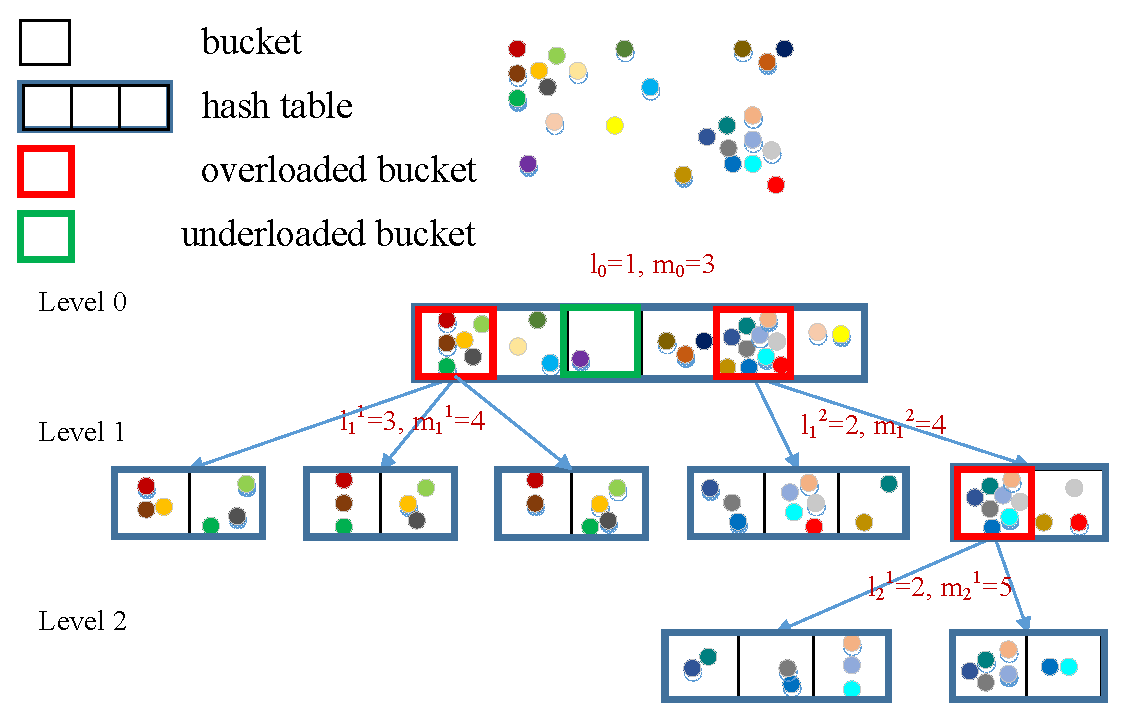
\includegraphics[width=3.2in]{fig/overview.eps}}
     \vspace{-0.05in}
    \caption{An illustrative example of LayerLSH structure (a bucket with more than 5 objects is considered as an overloaded bucket).}
    \label{fig:overview}
    \vspace{-0.2in}
\end{figure}

It is notable that since limiting bucket size will reduce the accuracy from probability theory's point of view (as shown in Equation (\ref{eq:prob})). The objects in the overloaded bucket should be copied to more than one hash tables to compensate for the reduced accuracy. This is for sustaining the expected accuracy $P$ as depicted in Equation (\ref{eq:prob2}), which will be described in detail in Section \ref{sec:layerlsh:param}. Since the overloaded buckets are rehashed recursively, multiple layers of LSH tables are constructed. The root level (level 0) of the LayerLSH is exactly the same as the original LSH. The hash tables in higher levels are the new generated LSH tables for the rehashed buckets. Figure \ref{fig:overview} shows an illustrative example of the \emph{\textbf{multi-layered}} tree-like structure.

%When an overloaded bucket is split, $l$ independent \emph{child hash tables} are created, where the split bucket is referred to as \emph{parent bucket}. The points in the parent bucket are rehashed in these child hash tables. The contents (objects) of the child tables are copies of the parent bucket, so that the objects in the split bucket have $l$ copies. Not only the level-0 bucket can be split but also the overloaded buckets at higher levels. Therefore, a \emph{\textbf{multi-layered}} tree-like structure is formed.


\subsection{Building LayerLSH}
\label{sec:layerlsh:param}

We rebuild the original hash tables in terms of two factors, the user specified expected recall and precision. Let $\text{KNN}(q,O)$ denote the set of $k$NNs of $q$. Given a query $q$ and a set of objects $O$, an approximate $k$NN query algorithm returns a set of candidates $\mathcal{C}$. We have the \textbf{recall} $\alpha=\frac{|\mathcal{C}\cap \text{KNN}(q,O)|}{|\text{KNN}(q,O)|}$, which implies the accuracy, and the \textbf{precision} $\beta=\frac{|\mathcal{C}\cap \text{KNN}(q,O)|}{|\mathcal{C}|}$, which implies the efficiency. Given $\alpha$ and $\beta$, we study the lower/upper bound size of each bucket as follows.

\begin{prop}
\label{theorem:bucketsize}
\textbf{(Bucket Size Constraints)} When using LSH with $l$ hash tables to answer $k$NN query, with an expected recall $\alpha$ and an expected precision $\beta$, the bucket size $S$ of each hash table has the following constraints:
\begin{equation}\label{eq:bucketsize}
    k\cdot(1-\sqrt[l]{1-\alpha})\leq S\leq \frac{k}{\beta\cdot l}.
\end{equation}
\end{prop}
\begin{proof}
Suppose the LSH parameters are $\{l, m, w\}$. In each of the $l$ hash table, the expected size of the bucket that $q$ falls in is $\overline S=\sum_{o\in O}p(|q,o|,w)^{m}$ where $p(s, w)^m$ is defined in Equation (\ref{eq:prob}) and (\ref{eq:prob1}). Let $s_{(q,k)}$ denote the distance from $q$ to its $k$th NN. Then we have
\begin{equation}\label{eq:recall2}
\begin{aligned}
  \overline S=\sum_{o\in O}p(|q,o|,w)^{m}&\geq \sum_{o\in \text{KNN}(q,O)}p(|q,o|,w)^{m}\\
                                        &\geq k\cdot p(s_{(q,k)},w)^m\\
                                        &\geq k\cdot(1-\sqrt[l]{1-\alpha}),
\end{aligned}
\end{equation}
The first ``$\geq$'' is true because the candidates for summation is reduced from $O$ to $\text{KNN}(q,O)$. The second ``$\geq$'' is true because for any $|q,o|\leq s_{(q,k)}$ we have $p(|q,o|,w)\geq p(s_{(q,k)},w)$ according to Equation (\ref{eq:prob}). The third ``$\geq$'' is true because in order to achieve the overall recall $\alpha$ over $l$ hash tables, the probability that $q$ and any of its $k$NNs collide in a specific hash table should be no less than $1-\sqrt[l]{1-\alpha}$ according to Equation (\ref{eq:prob2}). If we can make $p(s_{(q,k)},w)^m\geq 1-\sqrt[l]{1-\alpha}$ for $q$'s $k$th NN, it is also true for any other $k$NNs. Thus, the bucket size $S$ should satisfy $S\geq k\cdot(1-\sqrt[l]{1-\alpha})$.

When all of $q$'s $k$NNs are contained in the returned candidates set, i.e., $\text{KNN}(q,O)\subset\mathcal{C}$, $|\mathcal{C}|$ can be as large as $\frac{k}{\beta}$ to satisfy the expected precision, otherwise $|\mathcal{C}|$ has to be smaller. Thus, $\frac{k}{\beta}$ is the upper bound of $|\mathcal{C}|$. Since there are $l$ hash tables, the candidates are retrieved from $l$ buckets. Let us assume the candidates are collected evenly from $l$ hash tables. Thus, the bucket size $S$ should satisfy $S\leq \frac{k}{\beta\cdot l}$.
\end{proof}

Note that, satisfying the above constraints does not necessarily guarantee the expected recall and precision but helps us identify the underloaded and overloaded buckets.

Given the constraints of the bucket size, we propose Algorithm \ref{alg:split} to recursively rehash the overloaded buckets to build LayerLSH index. The input includes the original LSH tables (i.e., level-0 hash tables), the LSH parameters set $\{l,m,w\}$, the number of returned NNs $k$, the expected recall $R=\alpha$, and the expected precision $P=\beta$. With respect to each hash table, the recall is relaxed to $R'=1-\sqrt[l]{1-R}$, and the precision is tightened to $P'=P\cdot l$ (Line 2). Then, we have the lower bound size ($T_l=k\cdot R'$) and upper bound size ($T_u=\frac{k}{P'}$) for each bucket (Line 3). We check the size of each bucket of each hash table. For the overloaded bucket that contains more than $T_u$ objects (Line 7), we first determine a new set of child LSH parameters (Line 8), based on which the objects in that bucket are rehashed into a new set of hash tables (Line 9). The overloaded buckets are rehashed by recursively invoking this process until no bucket is overloaded (Line 10). For the underloaded bucket that contains fewer than $\frac{k\cdot\alpha}{l}$ objects (Line 11), we mark it for future use in query processing (Line 12).

\SetAlFnt{\small\sffamily}
\SetInd{0.55em}{0.5em}
\setlength{\textfloatsep}{0pt}
\begin{algorithm}[t]
\SetNoFillComment
\SetKwProg{Fn}{Function}{:}{end}
\SetKwFunction{RecSplit}{RecursSplit}\SetKwFunction{FindLSHParam}{FindParam}\SetKwFunction{LSH}{LSH}
\SetKwInOut{Input}{input}\SetKwInOut{Output}{output}

\Input{LSH hash tables $HT=\{HT_1,\ldots,HT_l\}$, LSH parameters $\{l,m,w\}$, $k$, $R=\alpha$, $P=\beta$}
\Output{LayerLSH hash tables set}
\BlankLine
\Fn{\RecSplit{$HT$, $\{l,m,w\}$, $R$, $P$}}{\
    $R'=1-\sqrt[l]{1-R}$, $P'=P\cdot l$\;
    $T_l=k\cdot R'$, $T_u=\frac{k}{P'}$\;
    \ForEach{$HT_i$ in $HT$}{
        \ForEach{bucket $b$ in $HT_i$}{
            $S\leftarrow$ size of $b$\;
            \If{$S>T_u$}{
                $\{l_c,m_c,w_c\}\leftarrow$\FindLSHParam($\{l,m,w\}$, $S$, $P'$)\;
                $HT_{child}\leftarrow$\LSH($b$, $\{l_c,m_c,w_c\}$)\;
                \RecSplit{$HT_{child}$, $\{l_c,m_c,w_c\}$, $R'$, $P'$};
            }
            \If{$S<T_l$}{
                mark $b$ as underloaded;
            }
        }
    }
}
\caption{Building LayerLSH}
\label{alg:split}
\end{algorithm}

In Algorithm \ref{alg:split}, we refer to the to-be-rehashed bucket as \emph{parent bucket} and the new LSH for this bucket as \emph{child LSH}. The core of bucket rehashing is to choose a proper new set of child LSH parameters, such that the bucket size is reduced (for efficiency) but at the same time the probability that a query and its $k$NNs collide in the same bucket is not reduced (for accuracy). We fix the LSH width parameter $w$. Let $\{l_p,m_p,w\}$ denote the set of parent LSH parameters, and $\{l_c,m_c,w\}$ denote the set of child LSH parameters. We use the following propositions to guide the selection of child LSH parameters.

\begin{prop}
\label{prop:accuracy}
\textbf{(For Accuracy)} Let $s_{(q,k)}$ denote the distance from a query $q$ to its $k$th NN. Suppose we can find a $r^*$ such that $r^*\geq s_{(q,k)}$ for any $q$. In order to NOT reduce the expected recall, the child LSH parameters $\{l_c,m_c\}$ should be chosen to satisfy:
\begin{equation}\label{eq:sustainprob}
    1-(1-p^{m_p+m_{c}})^{l_{c}}=p^{m_{p}},
\end{equation}
where $p=p(r^*,w)$ is defined in Equation (\ref{eq:prob}).
\end{prop}
\begin{proof}
Since $\forall q, r^*\geq s_{(q,k)}$, we have $p(r^*,w)^{m_p}\leq p(s_{(q,k)},w)^{m_p}$. That is, the probability that any query $q$ and its $k$th NN collide in the same bucket is no less than $p(r^*,w)^{m_p}$. If the probability $p(r^*,w)^{m_p}$ could be sustained after bucket rehashing, the probability that $q$ and any of its $k$NNs fall in the same bucket will not reduce, so that the expected recall $\alpha$ is guaranteed. Accordingly, in terms of Equation (\ref{eq:prob2}), the child LSH parameters $\{l_c,m_c,w\}$ should be chosen such that $1-[1-p(r^*,w)^{m_p+m_{c}}]^{l_{c}}\geq p(r^*,w)^{m_{p}}$. Further, since all the objects in child hash tables are originated from the parent bucket, the collision probability in child hash tables will never be greater than $p(r^*,w)^{m_{p}}$. Therefore, we aim to make $1-[1-p(r^*,w)^{m_p+m_{c}}]^{l_{c}}=p(r^*,w)^{m_{p}}$.
\end{proof}

In practice, $r^*$ can be approximately estimated by sampling. A number of sample objects are randomly selected to calculate their exact $k$NNs. The median of their $k$th NNs' distances is used to estimate $r^*$.

\begin{prop}
\label{prop:efficiency}
\textbf{(For Efficiency)} Let $S$ denote the size of the overloaded bucket that $q$ falls in. In order to approximately satisfy the precision constraint, the child LSH parameter $m_c$ and $l_c$ should be chosen as follows:
\begin{equation}\label{eq:forefficiency}
\begin{aligned}
    m_c&=\Big\lceil log_{p}\Big(\frac{k}{S\cdot\beta\cdot l_p}\Big)\Big\rceil,\\
    l_c&\leq\Big\lfloor\frac{k}{S_c^*\cdot\beta\cdot l_p}\Big\rfloor,
\end{aligned}
\end{equation}
where $p=p(r^*,w)$ is defined in Equation (\ref{eq:prob}), $\beta$ is the expected precision, and $S_c^*$ is the biggest bucket size among all child hash tables.
%Assume $S$ is approximately proportional to $X_{r^*}\cdot p(r^*,w)^m_{p}$, where $X_{r^*}$ is the exact number of objects whose distances to $q$ are less than $r^*$, i.e., $S\approx \gamma\cdot X_{r^*}\cdot p(r^*,w)^m_{p}$.
\end{prop}
\begin{proof}
The expected size of the bucket that $q$ falls in is $\overline S=\sum_{o\in O}p(|q,o|,w)^{m_p}$. From this equation, we learn that the actual bucket size relates to two factors, 1) the number of ``close'' objects to $q$ and 2) the probability that these ``close'' objects fall in $q$'s bucket (determined by $\{m_p,w\}$). The more ``close'' objects to $q$, the more likely $S$ is larger. The larger $m_p$ is, the more likely $S$ is smaller. Let $X=\{o:|q,o|\leq r^*\}$ denote the set of objects within a range of $r^*$, which are considered as ``close'' objects. In other words, $|X|$ implies $q$'s density. Then we assume that the bucket size $S$ is proportional to $|X|$, i.e., $S\propto |X|$. On the other hand, to simplify the analysis and obtain an approximate answer, we assume that the probability for all objects in $X$ falling in $q$'s bucket is proportional to $p(r^*,w)^{m_p}$ that is fixed for all objects in $X$, i.e., $S\propto p^{m_p}$ where $p=p(r^*,w)$. Thus, we have $S\propto|X|\cdot p^{m_p}$.

In order to satisfy the efficiency constraint $\frac{k}{S\cdot l_p}\geq\beta$, the bucket size $S$ should be reduced to less than $\frac{k}{\beta\cdot l_p}$. Since $S\propto|X|\cdot p^{m_p}$, $|X|\cdot p^{m_p}$ should be correspondingly reduced to $|X|\cdot p^{m_p+m_c}$. Therefore, we should choose $m_c$ to satisfy the following equation:
\begin{equation}\label{eq:forefficiency2}
    \frac{S}{\frac{k}{\beta\cdot l_p}}=\frac{|X|\cdot p^{m_p}}{|X|\cdot p^{m_p+m_c}}.
\end{equation}
Since $m_c$ should be an integer, we choose the result of the ceiling function, i.e., $m_c=\big\lceil log_{p}\big(\frac{k}{S\cdot\beta\cdot l_p}\big)\big\rceil$ to sustain the inequality of precision constraint.

On the other hand, after rehashing we also need to limit the number of child hash tables in order to satisfy the efficiency constraint. Suppose $S_{(q,i)}$ is the size of a query $q$'s bucket (or multiple child buckets if it points to child hash tables) in child hash table $i$, we need to make sure $\sum_{i=1}^{l_c}S_{(q,i)}\leq \frac{k}{\beta\cdot l_p}$. Further, suppose $S_c^*$ is the biggest bucket size among all child hash tables, we have $\sum_{i=1}^{l_c}S_{(q,i)}\leq l_c*S_c^*$. Thus, by making $l_c*S_c^*\leq\frac{k}{\beta\cdot l_p}$, i.e., $l_c\leq\big\lfloor\frac{k}{S_c^*\cdot\beta\cdot l_p}\big\rfloor$ (since $l_c$ should be an integer), we can satisfy the efficiency requirement.
\end{proof}

%Note that, $S_c^*$ is unknown before bucket rehashing. We will try a $l_c$ and rehash the bucket. If some buckets are still overloaded, the bucket rehashing process is invoked again. This is the reason why a recursive rehashing process is designed.

By combining Proposition \ref{prop:accuracy} and Proposition \ref{prop:efficiency}, we intend to obtain the available child LSH parameters $m_c$ and $l_c$, which are used during bucket rehashing (Line 8 in Algorithm \ref{alg:split}). However, there probably is no solution since the recall and precision requirements cannot be satisfied at the same time (i.e., $l_c$'s lower bound is greater than its upper bound). Furthermore, $S_c^*$ in Equation (\ref{eq:forefficiency}) is even unknown before bucket rehashing. In such a case, we first choose $m_c$ according to Equation (\ref{eq:forefficiency}), ignore the upper bound of $l_c$, and generate enough more child hash tables to sustain accuracy constraint according to Equation (\ref{eq:sustainprob}). We will further satisfy the efficiency constraint during the query processing.

%Specifically, we choose $m_c$ according to Equation (\ref{eq:forefficiency}). Thus, we will obtain $l_c$'s upper bound $\big\lfloor\frac{k}{S_c^*\cdot\beta\cdot l_p}\big\rfloor$ from Equation (\ref{eq:forefficiency}) and lower bound $\big\lceil log_{(1-p^{m_p+m_c})}(1-p^{m_p})\big\rceil$ from Equation (\ref{eq:sustainprob}). However, there probably is no solution since the recall and precision requirements cannot be satisfied at the same time (i.e., $l_c$'s lower bound is greater than its upper bound). In such a case, we ignore the upper bound of $l_c$ and generate enough more child hash tables to sustain accuracy constraint. We will further satisfy the efficiency constraint during the query processing.


\begin{comment}
\begin{equation}\label{eq:meanlc}
    \overline{l_c}=\Big\lceil\frac{\frac{k}{S_c^*\cdot\beta\cdot l_p}+log_{1-p^{m_p+m_c}}(1-p^{m_p})}{2}\Big\rceil
\end{equation}
\end{comment}

\begin{comment}
\begin{prop}
\label{prop:childparam}
\textbf{(Bucket Split-Child LSH Parameters)} In order to sustain the accuracy and efficiency, the bucket split should choose child LSH parameters as follows:
\begin{equation}\label{eq:sustainprob}
\begin{aligned}
    m_c&=m_p+\Big\lceil log_{p}\Big(\frac{k}{S\cdot\beta\cdot l_c}\Big)\Big\rceil,\\
    l_c&=\lceil log_{(1-p^{m_c})}{(1-p^{m_p})}\rceil,
\end{aligned}
\end{equation}
where $p=p(r^*,w)$. $w$ is consistent with parent LSH parameter.
\end{prop}
\end{comment}


\subsection{Query Processing}
\label{sec:layerlsh:query}

There are two kinds of buckets in LayerLSH, which should be differentiated during query processing. One kind that contains similar data objects, which are referred to as \emph{data buckets}. Another kind contains the pointers to child hash tables, which are referred to as \emph{pointer buckets}. In other words, in the LayerLSH tree-like structure, the leaf nodes are data buckets, while the internal nodes are pointer buckets.

\begin{algorithm}[t]
\SetNoFillComment
\SetKwProg{Fn}{Function}{:}{end}
\SetKwFunction{LayerLSHQuery}{LayerLSHQuery}
\SetKwInOut{Input}{input}\SetKwInOut{Output}{output}

\Input{query $q$, LayerLSH tables $HT=\{HT_1,\ldots,HT_l\}$, $k$, $R=\alpha$, $P=\beta$}
\Output{$k$NN candidates set $\mathcal{C}$}
\BlankLine
\Fn{\LayerLSHQuery($q$, $HT$, $R$, $P$, $\mathcal{C}$)}{\
    $\{l,m,w\}\leftarrow$ load LSH parameters for $HT$\;
    $R'=1-\sqrt[l]{1-R}$, $P'=P\cdot l$\;
    $T_l=k\cdot R'$, $T_u=\frac{k}{P'}$\;
    \ForEach{$HT_i$ in $HT$}{
        $b\leftarrow$ locate bucket with hash key $\{h_1(q),\ldots,h_m(q)\}$\;
        \If{$b$ is a pointer bucket}{
            $HT_{child}\leftarrow$ locate the child hash tables $b$ points to\;
            \LayerLSHQuery($q$, $HT_{child}$, $R'$, $P'$, $\mathcal{C}$);
        }
        \ElseIf{$b$ is a data bucket}{
            \If{$b$ is underloaded}{
                $B\leftarrow b$\;
                \While{$|B|<T_{l}$}{
                    $b'$ find ``nearby'' bucket from $b$\;
                    $B\leftarrow B\cup b'$;
                }
                $\mathcal{C}\leftarrow\mathcal{C}\cup B$;
            }
            \Else{
                \lIf{$R$ is primary}{$\mathcal{C}\leftarrow\mathcal{C}\cup b$}
                \lElseIf{$P$ is primary}{$\mathcal{C}\leftarrow\mathcal{C}\cup b'$ s.t. $|b'|\leq T_{u}$}
                \lElse{$\mathcal{C}\leftarrow\mathcal{C}\cup b'$ s.t. $|b'|\leq\frac{T_u+\frac{\sum_{i}^{l}|b_{(q,i)}|}{l}}{2}$}
            }
        }
    }
}
\caption{Query Processing in LayerLSH}
\label{alg:lshquery}
\end{algorithm}

To answer a $k$NN query, we use Algorithm \ref{alg:lshquery} to retrieve the candidates set from multi-layered hash tables. We first read the LayerLSH parameters $\{l,m,w\}$ from the input LayerLSH tables (Line 2). With respect to each hash table, the recall is relaxed to $R'$, and the precision is tightened to $P'$ (Line 3). Then, we have the lower bound size ($T_l=k\cdot R'$) and upper bound size ($T_u=\frac{k}{P'}$) for each bucket (Line 4). Given a query $q$, we first compute its compound hash keys and project $q$ to the bucket in a particular hash table (Line 6). If the positioned bucket is a pointer bucket, the query $q$ is rehashed in multiple child hash tables along with the bucket-based $R'$ and $P'$ (Line 8), and the query algorithm is invoked recursively (Line 9).


If the positioned bucket is a data bucket and this bucket is underloaded (Line 11), we will expand the search scope and search the ``nearby'' buckets whose compound hash keys are slightly different. This searching scope is expanded to more and more buckets as soon as enough objects ($T_l$) are returned (Line 12-16). The idea of merging ``nearby'' sparse buckets is similar to multi-probe LSH \cite{mplsh}. Given the property of LSH, if an object is close to a query $q$ but not hashed to the same bucket, it is likely to be in a bucket that is ``close by'' (i.e., the hash keys of the two buckets only differ slightly). LayerLSH also designates the ``close by'' buckets by applying a \emph{hash perturbation vector} $\Delta=\{\delta_1,\delta_2,\ldots,\delta_m\}$ (e.g., $\{+1,0,\ldots,0\}$ or $\{0,-1,\ldots,0\}$) on the original compound hash key $G(q)=\{h_1(q),h_2(q),\ldots,h_m(q)\}$ and obtains the nearby bucket $G(q)+\Delta$.

%However, multi-probe LSH performs nearby bucket searching without discrimination. The search of the dense bucket and its nearby buckets will return a large number of candidates but only with a limited accuracy improvement. In contrast, LayerLSH only searches for nearby buckets for sparse queries, which is more cost efficient.


If the data bucket is not underloaded, the objects in that bucket are conditionally put into the candidates set $\mathcal{C}$ (Line 17). Recall that, it is possible that the specified recall and precision are conflict with each other. It is required to return all candidates from all hash tables in order to satisfy the recall requirement, but also required to return at most $T_u$ candidates from only a few hash tables to satisfy the precision requirement. LayerLSH will let users specify one primary choice, the expected recall $\alpha$ or the expected precision $\beta$. Then the query processing algorithm will correspondingly include all the objects in bucket to satisfy recall requirement (Line 18) or limit the number of returned candidates to satisfy precision requirement (Line 19). If both or none of recall and precision is primarily selected, LayerLSH balances these two factors and return at most $\frac{T_u+\frac{\sum_{i}^{l}|b_{(q,i)}|}{l}}{2}$ candidates, where $T_u$ is for precision requirement and $\frac{\sum_{i}^{l}|b_{(q,i)}|}{l}$ is for recall requirement (where $b_{(q,i)}$ is $q$'s bucket in the $i$th child hash table).




\begin{comment}
\begin{figure}[htb]
    \centerline{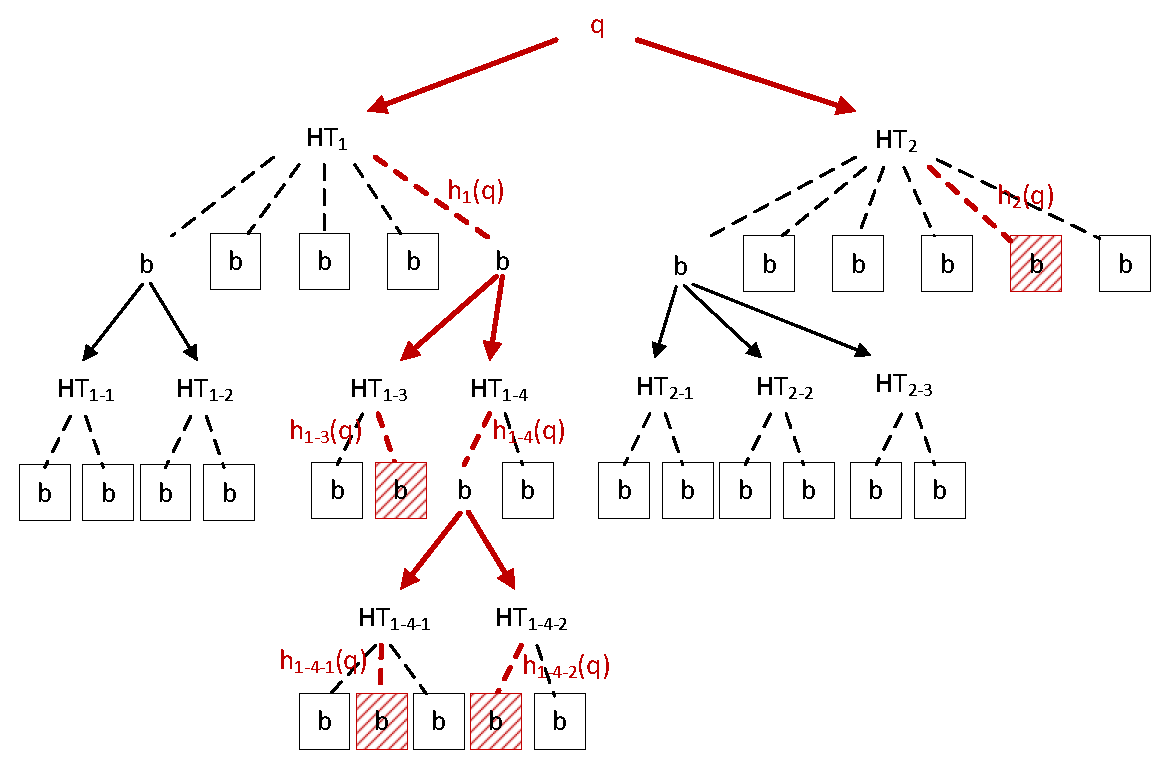
\includegraphics[width=3.2in]{fig/layerlshquery.eps}}
    \caption{Approximate $k$NN query in LayerLSH. HT denotes a hash table, and b denotes a bucket. The red lines or dashed lines show the query paths. The shadowed boxes are the data buckets which the query $q$ falls in.}
    \label{fig:layerlshquery}
\end{figure}
\end{comment}




It is noticeable that the query might expand to more and more buckets as it goes deeper in the LayerLSH tree. However, the large number of checked buckets does not necessarily lead to large number of candidates since the checked buckets are much smaller. With regard to the dense buckets, LayerLSH narrows the search scope, as a result the search is more efficient. Rather than using a large number of hash tables to achieve high search quality, we can achieve the same search quality with a smaller number of level-0 hash tables. More hash tables are only created for the dense buckets. The hashing is more targeted in terms of data distribution.

\begin{comment}
\subsection{Integrating Multi-Probe LSH}

The idea of multi-probe LSH \cite{mplsh} is simple but effective. Given the property of LSH, if an object is close to a query $q$ but not hashed to the same bucket as $q$, it is likely to be in a bucket that is ``close by'' (i.e., the hash values of the two buckets only differ slightly). Multi-probe LSH designates the ``close by'' buckets by applying a \emph{hash perturbation vector} $\Delta=\{\delta_1,\delta_2,\ldots,\delta_m\}$ on the original compound hash key $G(q)=\{h_1(q),h_2(q),\ldots,h_m(q)\}$ and obtains the nearby bucket $G(q)+\Delta$. Since similar objects should hash to the same or adjacent values (i.e., differ by at most 1), the original paper \cite{mplsh} suggests to only focus on perturbation vectors $\Delta$ with $\delta_i\in\{-1,0,1\}$.

%An $n$-step perturbation vector $\Delta$ has exactly $n$ coordinates that are non-zero. Intuitively, buckets that are returned by 1-step probing are more likely to contain objects that are close to the query object than buckets returned by 2-step probing. Therefore, the \emph{step-wise probing} first probes all the 1-step buckets, then all the 2-step buckets, and so on.

%The idea of multi-probe LSH is to expand the search scope of the relatively sparse bucket.
As illustrated in Section \ref{sec:intro}, queries that are projected to the bucket with low density suffers from the low accuracy problem. Increasing the number of hash tables would improve the search quality at the expense of more searching cost. In contrast, multi-probe LSH improves the search quality by searching nearby buckets. However, multi-probe LSH performs nearby bucket searching without discrimination. The search of the dense bucket and its nearby buckets will lead to high distance computation cost but only with a limited improvement.

LayerLSH integrates the idea of multi-probe LSH, which identifies the densities of buckets and performs more targeted nearby bucket search. That is, we only search for nearby buckets for sparse queries. Note that, there are multiple layers of buckets in LayerLSH. Since the nearby buckets are more similar at lower levels than at higher levels, when handling a sparse query the lower-level nearby buckets are given higher priority than the higher-level nearby buckets. The bucket search terminates until a predefined number of points is searched.

%the number of checked points is larger than $T$ where $T$ is the bucket limit in bucket split.


%Note that, multi-probe LSH is a probing optimization technique on the basic LSH index structure instead of a new indexing scheme. We will use it to optimize our query process in the paper.

%The original paper shows that most $k$ nearest neighbors are retrieved by only probing 1-step buckets and 2-step buckets.
\end{comment}

need to discuss non-fix w

\subsection{Index Maintenance}

supporting dynamic data, using lsm-like technique

disk based index should be more detailed

LayerLSH can be implemented as a disk-based index for maintaining large data sets. Since the basic structure in LayerLSH is tree-like, it is straightforward to store the index using a tree structure. The internal nodes storing the child LSH parameters as well as the pointers to child buckets are maintained in an \emph{index file}, and the leaf nodes storing the data points are maintained in a \emph{data file}. Note that, one leaf nodes that stores a large bucket is written to multiple file blocks, and multiple leaf nodes storing multiple small buckets are written to a single file block to save space. Similar buckets are stored continuously in a file block to support ``nearby'' bucket search.

When answering queries, the internal nodes maintained in index file are loaded into memory for fast access, or part of them for large index. After the data buckets are positioned, the file blocks storing the candidate buckets are loaded into memory for distance measurements, followed by returning the approximate $k$NNs. To support insertion of a point, we first locate the file blocks that store the hashed buckets and then append the point data. Note that, request of a new file block might be needed if the returned file block is full. To support deletion of a point, we first locate the file blocks and label this point indicating its invalidation. A periodical recycling process is executed offline to recycle the file blocks where no valid data is contained.

\subsection{Complexity Analysis}












%\section{LayerLSB: Rebuild LSB-Tree}
\label{sec:reclsb}

In this section, we rebuild another representative index structure LSB-tree by exploring the density of hash values.


\subsection{LSB Background}
\label{sec:reclsb:review}

The LSB approach constructs an LSB-tree structure and performs approximate NN queries by exploiting the tree structure \cite{lsb}. Each multi-dimensional object $o$ is reduced to a 1-d $z$-value $z(o)$ \cite{Gaede:1998:MAM:280277.280279}. The multi-dimensional objects can be organized in the numerical order of their $z$-values and are indexed by a conventional B-tree. The close points in high dimensional space exhibit similar $z$-values, so that the $k$-NN search for a query $q$ is translated into one dimensional range search on the $z$-values around query $q$'s $z$-value. This is the basic idea of LSB-tree. In addition, multiple LSB-trees can be built to improve search quality.

%First, each $d$-dimensional data object $o$ is converted to a $m$-dimensional object $G(o)=\{H_1(o), H_2(o), \ldots, H_m(o)\}$ where $H_i(o)=a\cdot o+b^*$. Here, $a$ is a $d$-dimensional vector where each component is drawn independently from the normal distribution. Value $b^*$ is uniformly distributed in $[0,2^{\lceil log_{2}dt\rceil}w^2)$, where $t$ is the largest coordinate on each dimension and $w$ is the partition width. Then, each $G(o)$ is regarded as a point in a $m$-dimensional space, and its \emph{$z$-value} $z(o)$ can be derived based on \cite{Gaede:1998:MAM:280277.280279}. Basically, the $z$-value of a $G(o)$ is calculated by interleaving the binary representations of $G(o)$'s coordinate values from the most significant bit to the least significant bit. For example, given a 4-d object $o$ (29, 8, 78, 34), it is first converted to a 2-d object $G(o)=\{H_1(o),H_2(o)\}=(2,5)$, and the binary representation of $G(o)$'s coordinates is (010,101). Then, its $z$-value is $z(o)=011001$ (i.e., 25).

%In such a way, a multi-dimensional object is reduced to a 1-d $z$-value. The multi-dimensional objects can be organized in the numerical order of their $z$-values and are indexed by a conventional B-tree. The close points in high dimensional space exhibit similar $z$-values, so that the $k$-NN search for a query $q$ is translated into one dimensional range search on the $z$-values around query $q$'s $z$-value. This is the basic idea of LSB-tree. In addition, multiple LSB-trees can be built to improve search quality.

Let us focus on the query process in LSB-tree. The approximate $k$-NN query is achieved by a synchronous bi-directional expansion at the leaf levels of all LSB-trees. For a given query $q$, its $z$-value $z_j(q)$ in each LSB-tree $T_j(1\leq j\leq l)$ is first computed. The closeness between two $z$-values is captured by the notion of \emph{Length of the Longest Common Prefix} (LLCP) \cite{lsb}. We search each $T_j$ to locate the leaf node whose $z$-value is the closest to $z_j(q)$. The query algorithm examines the leaf's left sibling and right sibling (which are supposed to be similar objects to $q$), and proceeds through a synchronous bi-directional expansion of all trees in decreasing order of their LLCP with $z_j(q)$. The expansion is terminated in terms of any of the two proposed termination conditions, $E_1$: the total number of leaf entries accessed from all $l$ LSB-trees has reached $4Bl/d$ where $B$ is the page size; $E_2$: the nearest point found so far has distance to $q$ at most $2^{u-\lfloor v/m\rfloor+1}$ where $u$ is fixed for each dataset and $v$ is its LLCP with $z_j(q)$, by which the search quality can be guaranteed. If the quality is not necessarily guaranteed, users can also just terminate it when a pre-defined number of expansions is reached.

%The LSB approach maintains LSH index by constructing a B-tree structure. SK-LSH shares the similar idea and also constructs a B-tree structure but with different dimension reduction method \cite{sklsh}. We will reconstruct the LSB-tree structure by exploring the density of leaf entry values. We believe that similar reconstruction could also be applied to the SK-LSH's B-tree stucture.

%The LSB approach relies on the basic idea that similar data objects tend to have similar $Z$-values. The similarity between two $Z$-values (reflecting the similarity between two data objects) is captured by

\subsection{LayerLSB Structure}

LSB projects the original high dimensional points to 1-d $z$-values. The skewed data distribution leads to skewed distribution of $z$-values. From the LSB-tree's perspective, the neighboring leaf nodes with relatively large $z$-value difference (i.e., small LLCP) are referred to as \emph{loose neighbors}, while those with relatively small $z$-value difference are (i.e., large LLCP) referred to as \emph{tight neighbors}. A pair of loose neighbors indicates that their corresponding original data points are likely far away from each other, while tight neighbors probably indicates close points. As shown in Figure \ref{fig:dens:lsb}, the quality of approximate $k$-NN query has correlation with the leaf neighbors' tightness which is quantified by range density. It exhibits high search quality when the query point resides in a range of loose neighbors (i.e., low range density) and low search quality when it resides in a range of tight neighbors (i.e., high range density). This is owing to the inherent drawback of $z$-values. The $z$-values traversal sometimes returns far apart point when it moves to another region indexed by another most significant bit \cite{zorkderknn,Zhang:2012:EPK:2247596.2247602}, and this error will be amplified in the dense ranges as explained in Section \ref{sec:intro}.

%This phenomenon can be explained as follows. The approximation for query in low density range is usually with larger LLCP. Accordingly, an erroneous approximation in low density range with large LLCP to query tends to return a far-away point, which has greater impact on the search quality. Even though the $E_2$ termination condition guarantees a given approximation ratio by considering a candidate's LLCP ($E_1$ does not consider LLCP), the bi-directional expansion search terminates when it first meets a candidate that satisfies the condition, and another much closer point could be missed.

\begin{figure}[t]
    \centerline{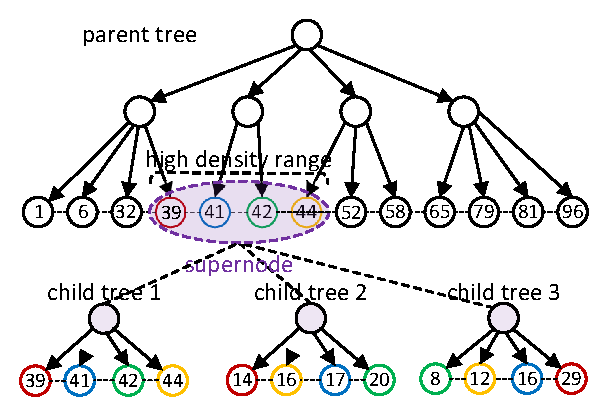
\includegraphics[width=2.8in]{fig/layerlsb.eps}}
    \caption{An illustrative example of LayerLSB structure. The circles with the same color indicate the same original data point. The number inside each circle is the $z$-value of that point in a particular LSB-tree.}
    \label{fig:layerlsb}
\end{figure}

We propose LayerLSB structure by exploring the density of $z$-values. Since the queries falling in high density range usually show low search quality, extra efforts are put into building indices for these queries. Figure \ref{fig:layerlsb} shows an illustrative example of LayerLSB structure. The leaf nodes in high density ranges are rehashed in multiple independent child LSB-trees. These leaf nodes in parent tree are merged as a \emph{supernode}. The original $z$-value\footnote{The common representation of a $z$-value is a binary string. For ease of exposition, we use a positive integer to represent a binary string for demonstrating the tightness of leaf entries.} obtained in parent LSB-tree are retained in the first child tree. Two extra child trees with a new set of LSB parameters are further created. As a result, new $z$-values of these rehashed data points are obtained.

Even though only two levels are shown in Figure \ref{fig:layerlsb}, it is possible to further rehash the level-1 child LSB leaf nodes and create level-2 child LSB-trees. This results a \emph{multi-layered} LSB-trees structure. This variation of $z$-values' order achieved by extra LSHs will increase the probability of returning real $k$NNs. Comparing to blindly createing more LSB-trees without discrimination, great effort can be saved by targeted rehashing. A small number of root level LayerLSB-trees is enough to obtain a high search quality. Next, we will describe how to build the LayerLSB structure.


\subsection{Building LayerLSB-Tree}

\Paragraph{Range Density Evaluation} To rebuild LSB-tree, evaluating the tightness of leaf neighbors is the first step. Recall that each leaf node is designated with a $z$-value. We use \emph{z-value range density} to quantify the tightness of leaf neighbors. It is straightforward to make a histogram to estimate the range densities where the length of each bin indicates the number of $z$-values in that range. Thus, the leaf nodes in dense ranges can be identified for further rehashing.

\Paragraph{Child LSB Parameters Determination} The identified high density leaf nodes are going to be inserted into multiple independent child LSB-trees. With respect to the parameters setting in child LSB, the dimensionality $m_{c}$ of $G(o)$ is set as $m_{c}=log_{1/p_2}{\frac{dn}{B}}$ (where $p_2$ is a constant probability under an approximation ratio and $B$ is the page size for external storage) \cite{lsb} and the partition width is consistent with its parent tree. Since the number of child tree points $n$ is much smaller than that in parent tree, $m_{c}$ is a small number, and the length of each $z$-value is greatly reduced. This results in a smaller index for child LSB-trees. In addition, we leave the number of child trees $l_{c}$ as a user-defined parameter as it balances the tradeoff between search quality and search cost.
%We will empirically show the effect of $l_{c}$ in Section \ref{sec:expr:param}.

\Paragraph{Child LSB-Tree Generation} With regard to every point in a high density range, a number $l_{c}$ of $z$-values are computed and inserted into these child LSB-trees respectively. The child tree generation process is executed recursively until no dense range exists. It is noticeable that too many levels will take up too much space and degrade query performance. Fortunately, it is common that only one child LSB level is enough to achieve high search quality.


\subsection{Query Processing}

%The query processing in LayerLSB is a simple extension of the that in original LSB. We first review the query processing in the original LSB. The LSB uses the \emph{length of the longest common prefix} (LLCP) of $z(q)$ and $z(o)$ denoted by $LLCP(z(q), z(o))$ to quantify the similarity of two $Z$-value $z(q)$ and $z(o)$. Recall that the $Z$-value $z(o)$ is a binary string. The larger of the $LLCP(z(q), z(o))$ is, the more likely that $o$ is similar to $q$. The nearest neighbor algorithm in original LSB performs a synchronous bi-directional expansion at the leaf levels of all trees and visits leaf entries in descending order of their LLCPs to $z(q)$.

\begin{algorithm}[t]
\SetKwData{Query}{$q$}\SetKwData{Heap}{$H$}\SetKwData{Entry}{$e$}\SetKwData{CandidateSet}{$S$}
\SetKwProg{Fn}{Function}{:}{end}
\SetKwFunction{FindEntryInTrees}{FindNodeInTrees}
\SetKwInOut{Input}{input}\SetKwInOut{Output}{output}

\Input{query \Query, LayerLSB trees $\{T^0_1,T^0_2,\ldots,T^0_l\}$}
\Output{$k$NN candidates set \CandidateSet}
\BlankLine
initialize a min-heap \Heap and a set \CandidateSet\;
\FindEntryInTrees(\Query, $\{T^0_1,T^0_2,\ldots,T^0_l\}$, \Heap)\;
\While{not terminated}{\
    \Entry $\leftarrow$ \Heap.pop()\;
    insert \Entry into \CandidateSet\;
    \tcc{from parent tree to child trees}
    \uIf{\Entry.next is a supernode}{\
        \FindEntryInTrees(\Query, \Entry.next.ctrees, \Heap)\;
    }
    \tcc{from child tree to parent tree}
    \uElseIf{\Entry.next is left/right-most leaf node}{\
        \If{\Entry.supernode is not null}{\
            push \Entry.supernode.next into \Heap\;
        }
    }
    \Else{
        push \Entry.next into \Heap\;
    }
}
return \CandidateSet;
\BlankLine
\BlankLine
\Fn{\FindEntryInTrees{\Query, $\{T_1,T_2,\ldots\}$, \Heap}}{\
    \ForEach{$T_i$ in $\{T_1,T_2,\ldots\}$}{\
        compute $z_i(\Query)$ in $T_i$\;
        \eIf{$z_i(\Query)$ belongs to a supernode}{\
            \FindEntryInTrees(\Query, supernode.ctrees, \Heap)\;
        }{
            locate $e\vdash_i$ and $e\dashv_i$ in $T_i$ based on $z_i(\Query)$\;
            push $e\vdash_i$ and $e\dashv_i$ into \Heap\;
        }

    }
}
\caption{The $k$NN algorithm in LayerLSB}
\label{alg:layerlsb_query}
\end{algorithm}

The query processing in LayerLSB is similar to that in original LSB. Both rely on bidirectional expansion. But there is a key difference between them, which is that in LayerLSB the expansion might move between parent tree and child trees. We describe the query algorithm of LayerLSB in Algorithm \ref{alg:layerlsb_query}.

We use a min-heap $H$ to maintain the leaf nodes in descending order of their LLCP with $q$ (Line 1). Denote the $l$ root-level (or level-0) LSB-trees as $T^0_1,T^0_2,\ldots,T^0_l$ respectively. We first search each root-level tree $T^0_i$ to locate the leaf node $e\vdash_i$ with the lowest $z$-value at least $z_i(q)$ (i.e., right-moving node) and the leaf node $e\dashv_{i}$ with the highest $z$-value at most $z_i(q)$ (i.e., left-moving node and preceding node of $e\vdash_i$) (Line 23,24). If $z_i(q)$ falls into a high density range, i.e., $z_i(q)$ belongs to a supernode that links to multiple child trees, we will recursively compute $q$'s $z$-values in child trees and locate the corresponding left-moving and right-moving nodes that will be pushed into $H$ (Line 21).

Next, we pop the first node $e$ from $H$ which has the largest LLCP with $q$ (Line 4). The moving direction information is embedded in node $e$ such that $e$.next will return $e$'s left-sibling node or right-sibling node. If $e$.next falls into a low density range, i.e., $e$.next belongs to a supernode and links to multiple child trees, we should move the cursor from parent tree to child trees. A recursive \texttt{FindNodeInTrees} process is invoked to search leaf nodes in child trees (Line 6). If $e$.next happens to be the left-most/right-most node of the tree, which means that all the leaf nodes preceding/following $z(q)$ have been visited in that tree, we should move the cursor from child tree to parent tree unless it is already root-leveled. The left/right sibling leaf node of the supernode where $e$ falls is pushed into heap $H$ (Line 10). Otherwise, $e$.next is a leaf node at the same level as $e$ such that $e$.next is simply pushed into $H$. This bidirectional expansion process continues until a certain termination condition is satisfied. All the popped nodes from $H$ are considered as $k$-NN candidates and returned for further distance measurement.

\begin{comment}
\begin{figure}[htb]
    \centerline{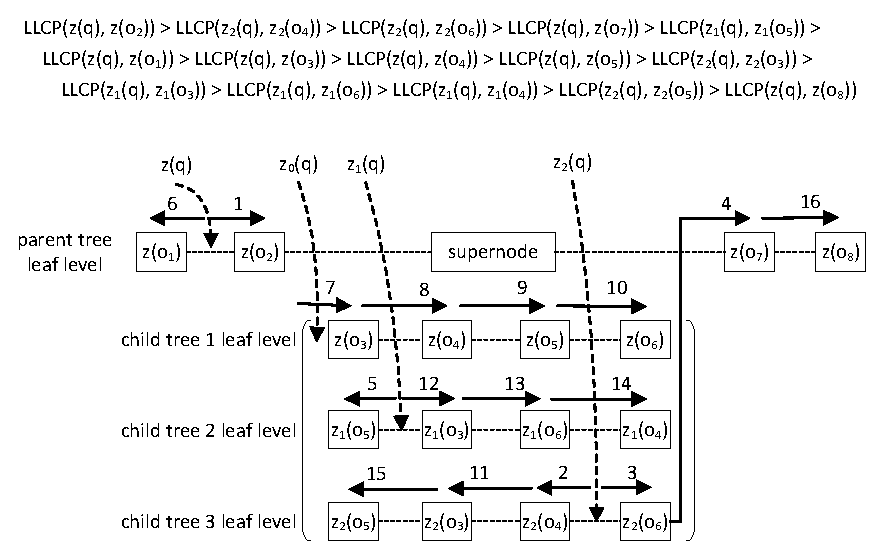
\includegraphics[width=3.4in]{fig/layerlsb_query.eps}}
    \caption{An illustrative example of query process in LayerLSB with a single parent tree and 3 child trees. The upper part shows the global LLCP order in both parent tree and child trees. We move left or right one position each step. The number above the moving direction means the moving step. }
    \label{fig:layerlsb_query}
    \vspace{-0.1in}
\end{figure}

Figure \ref{fig:layerlsb_query} shows an illustrative example. Only the leaf levels of parent tree and child trees are drawn. The supernode at parent tree level links to the 3 child trees. The moving between parent tree and child trees should be noticeable. 1) When moving from parent tree to child trees, new $z$-values of $q$ are computed with child LSB parameters, and the LLCPs with left/right sibling node in child trees should be reevaluated. 2) When moving from child tree to parent tree, the parent-level node is visited only for the first time from child tree to parent tree, since multiple child trees linked from the parent tree.
\end{comment}

Note that, the query in LayerLSB structure will not impact LSB's theoretical quality guarantee. We just create more targeted child trees for part of the parent tree. As long as we sustain the termination condition $E_1$ and $E_2$, the collision probability will not be impacted.

%\Paragraph{Quality Guaranteed Approximate Query Processing}
%The original LSB endows with a very good property that performs approximate NN query with quality guarantee. This is achieved by carefully setting parameters and fulfilling termination condition $E_1$ and $E_2$ as discussed in Section \ref{sec:reclsb:review}. To guarantee search quality with the multi-level tree structure in LayerLSB, we accordingly set LSH parameters and sustain the termination condition $E_1$ and $E_2$. The parameters of level-0 LSB trees are set consistent with the original LSB, i.e., $l=\sqrt{dn/B}$ and $m=log_{1/p2}(dn/B)$. With regard to the higher level trees, $m$ is set the same as level-0 tree, and $l$ is a user-specified number. It is obvious that as long as the same termination condition $E_1$ and $E_2$ are fulfilled, the expected quality of LayerLSB is no lower than the original LSB no matter what $l$ is. To satisfy $E_1$, we ensure that the number of leaf entries accessed from all level-0 trees plus the number of unique leaf entries accessed from all child trees has reached $4Bl/d$. On the other hand, we can assure $E_2$ by ensuring that the nearest point found so far has distance to $q$ at most $2^{u-\lfloor v/m\rfloor+1}$.

\begin{comment}
\subsection{Index Maintenance}

LSB-tree is originally a disk-based index. The core is a B-tree structure. For supporting bidirectional expansion operation, the leaf node stores pointers to its left sibling and right sibling. The insertion and deletion are well supported in the conventional B-tree structure. LayerLSB index structure follows the design of LSB. Besides, 1) for supporting the moving operation between parent tree and child trees, the left/right neighbor node of a supernode stores pointers to the leftmost/rightmost nodes of child trees, and vice versa. In addition, 2) the leaf node (with $z(o)$) contained in a supernode stores pointers to its corresponding leaf nodes (with $z_j(o)$) in child trees, so the location of a query in multiple child trees can be achieved through much fewer I/O operations.
\end{comment}


\section{Applicability to Other LSH Indices}
\label{sec:extension}

We discuss the possibilities of applying our approach to other LSH variants in this section.

%As long as the basic index structure is a hash table or B-tree, it is possible to rebuild the index with multi-layered structure by leveraging density of hash values.
\subsection{Table-based LSH and LayerDSH}
\label{sec:extension:dsh}

The idea of rehashing points with multi-layered structure should work as long as the basic index structure is a hash table.
%The data points in heavy loaded buckets can be reorganized to achieve better performance.
For example, \textbf{C2LSH} \cite{c2lsh} randomly chooses a number of LSH functions to form a function base and performs $k$NN query based on the intuition that a query $q$ should collide with its close neighbors under a large number of LSH functions. Though the idea is novel, the basic indexing structure is a hash table, so that we can reorganized the points in dense buckets using the multi-layered structure to improve efficiency. In addition, \textbf{DSH} \cite{Gao:2014:DDS:2588555.2588565} and \textbf{Selective Hashing} \cite{Gao:2015:SHC:2783258.2783284} were recently proposed to address the unbalanced data distribution problem, which can also integrate the multi-layered structure to further balance the hash table. We briefly demonstrate the idea of rebuilding DSH as follows.

%However, how to guarantee the search quality after integrating multi-layered structure is an open problem for these LSH variants.

\Paragraph{LayerDSH} DSH \cite{Gao:2014:DDS:2588555.2588565} aims to build data-sensitive hash family for the skewed data and directly answers $k$NN query. The DSH family is defined as follows \cite{Gao:2014:DDS:2588555.2588565}:
\begin{definition}
\label{def:dsh}
(\textbf{DSH family}) A family $\mathcal{H}=\{h:R^d\rightarrow\{0,1\}\}$ is called $(k,ck,p_1,p_2)$-sensitive if for any query point $q\in R^d$ and $o\in O$
\begin{itemize}
  \item If $o\in NN(q,k)$ then $\frac{|\{h|h(o)=h(q),h\in\mathcal{H}\}|}{|\mathcal{H}|}\geq p_1$,
  \item If $o\notin NN(q,ck)$ then $\frac{|\{h|h(o)=h(q),h\in\mathcal{H}\}|}{|\mathcal{H}|}\leq p_2$.
\end{itemize}
\end{definition}
The DSH family can be learned from the data and generated by combining adaptive boosting and spectral techniques \cite{Gao:2014:DDS:2588555.2588565}, which is endowed with good theoretical guarantee.

Even though the points are distributed more evenly and the buckets are more balanced in DSH than that in LSH, the buckets are not totally balanced as shown in the experimental results \cite{Gao:2014:DDS:2588555.2588565}. As DSH aims to generate proper hash families to generate balanced hash tables, our idea can be applied to the DSH tables as a postprocessing step to further balance the hash tables. We propose LayerDSH which rehashes the dense buckets and merges the sparse buckets for DSH. The building process of LayerDSH is similar to LayerLSH. According to the definition of DSH, the expected recall $\alpha$ should be set as $\alpha=p_1$ which is defined in Definition \ref{def:dsh}. In addition, to sustain the success probability, the probability $p$ appeared in Proposition \ref{prop:accuracy} and \ref{prop:efficiency} should be set as $p=p_1$ instead of $p=p(r^*,w)$.


\subsection{Tree-based LSH and LayerLSB}

There exist several tree-based LSH index structures, such as LSB \cite{lsb}, LSH Forest \cite{Bawa:2005:LFS:1060745.1060840}, and SK-LSH \cite{sklsh}. \textbf{LSH Forest} \cite{Bawa:2005:LFS:1060745.1060840} exploits tree structure to manage hash values. Each hash function applied on an object produces one bit. Each object is assigned with a label containing a sequence of bits that are generated from multiple hash functions, such that the close points are assigned with similar labels. Since the sequence of bits can be linearly ordered, they are indexed by a tree. A collection of multiple LSH trees forms a \emph{LSH Forest}. \textbf{SK-LSH} \cite{sklsh} defines a new distance measure of two hash values which captures the similarity of two points, so that the hash values can be linearly ordered and indexed by B-tree structure. By exploring the density of hash values, both of the two tree-based LSH indices can be rebuilt with multi-layered structure.


\Paragraph{LayerLSB}
The \textbf{LSB} approach constructs an LSB-tree structure and performs approximate NN queries by exploiting the tree structure \cite{lsb}. Each multi-dimensional object $o$ is reduced to a one-dimensional $z$-value $z(o)$ \cite{Gaede:1998:MAM:280277.280279}. The multi-dimensional objects can be organized in the numerical order of their $z$-values and are indexed by a conventional B-tree. The close points in high dimensional space exhibit similar $z$-values, so that the $k$NN search for a query $q$ is translated into one dimensional range search on the $z$-values around query $q$'s $z$-value. This is the basic idea of LSB-tree. In addition, multiple LSB-trees can be built to improve search quality. The approximate $k$NN query is achieved by a synchronous bi-directional expansion at the leaf levels of all LSB-trees.

\begin{figure}[t]
\vspace{-0.1in}
    \centerline{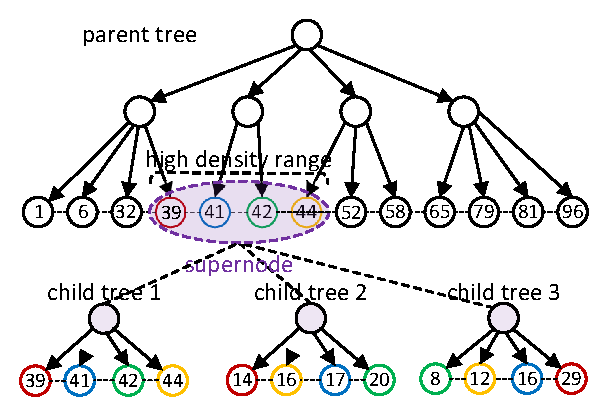
\includegraphics[width=2.6in]{fig/layerlsb.eps}}
    \caption{An illustrative example of LayerLSB structure. The circles with the same color indicate the same original data point. The number inside each circle is the $z$-value of that point in a particular LSB-tree.}
    \label{fig:layerlsb}
\end{figure}

We propose LayerLSB structure by exploring the density of $z$-values. Since the queries falling in high density ranges usually exhibit low search quality, extra efforts are put into building indices for these queries. Figure \ref{fig:layerlsb} shows an illustrative example of LayerLSB structure. The leaf nodes in high density ranges are rehashed in multiple independent child LSB-trees. These leaf nodes in parent tree are merged as a \emph{supernode}. The original $z$-values obtained in parent LSB-tree are retained in the first child tree. Two extra child trees with a new set of LSB parameters are further created. As a result, new $z$-values of these rehashed data points are obtained.

Even though only two levels are shown in Figure \ref{fig:layerlsb}, it is possible to further rehash the level-1 child LSB leaf nodes and create level-2 child LSB-trees. This results in a \emph{multi-layered} LSB-trees structure. This variation of $z$-values' order achieved by extra LSHs will increase the probability of returning the real $k$NNs. Comparing to blindly creating more LSB-trees without discrimination, great efforts can be saved by targeted rehashing. A small number of root level LayerLSB-trees is enough to achieve high search quality.

\section{Distributed Implementation}
\label{sec:distributed}

\Paragraph{Distributed LSH} The approach of supporting distributed NN search with both LSH and LayerLSH is straightforward. Suppose we have $n$ workers. A bucket with key $bk$ is assigned to worker $\frac{H(bk)}{n}$ where $H(\cdot)$ is any hash function that maps a bucket key to an integer. As a query $q$ arrives, its multiple hash values $G_1(q), G_2(q), \ldots, G_l(q)$ corresponding to multiple hash tables are first calculated. The query is then sent to multiple workers $\frac{H(G_j(q))}{n}, 1\leq j\leq l$ for local computation. The candidates obtained by local NN search are refined before being merged as a global candidate list, where the refining method could be extracting only the top $k$ nearest neighbors. Due to the skewed data distribution, hot spots might exist in distributed LSH, while LayerLSH has the advantage of alleviating hot spot contention.

\begin{comment}
\Paragraph{LSB and LayerLSB} The basic idea of NN search in LSB is bidirectional expansion on an ordered $z$-values list. In distributed implementation, it is intuitive to split the $z$-values list by range partition and let each worker serve for a range of the list. However, hot spots might exist due to skewed data distribution. We assign the dense ranges to additional workers to distribute the heavy workload. Upon receiving a query request, the worker routes the query to additional workers, such that the heavy workload can be shared by redundant workers. Considering the high synchronization cost in distributed processing, a set of local neighbors are returned rather than only one at each time. Similarly, in distributed LayerLSB, the child trees' $z$-values are also split by range partition and allocated to additional workers. Upon receiving a query request, the worker that holds the parent tree first compute its $z$-values with child LSB base, and routes the query to the corresponding workers where the $z$-values are covered.
\end{comment}

\Paragraph{All-Pairs Computation} All-pairs computation is a common preprocessing step in many applications, e.g., retrieving similarity matrix for learning data correlations \cite{allpair1}, pruning distant neighbors for abstracting a graph structure \cite{ap}, evaluating implicit properties for each data point \cite{lshcluster}, and so on. All-pairs computation is known as a computation intensive task, which requires $N^2$ distance measurements. This is extremely costly for large volume and high dimensional data. Since the all-pairs computation is often performed only based on the nearest neighbors in these applications, LSH is an ideal approximation method to optimize all-pairs computation. Furthermore, using distributed machines can further speedup the computation intensive task. The LSH buckets are distributed among multiple workers, where the all-pairs computation is performed locally within each bucket.

However, distributed LSH-based all-pairs computation suffers from the drawback of skewed bucket size distribution. The workers with dense buckets can be the stragglers, which can significantly slow down the whole process. Fortunately, LayerLSH can alleviate this impact by bounding the bucket size, while at the same time guaranteeing the accuracy. Moreover, we merge similar small buckets in order to not only improve the accuracy but also reduce the number of distributed tasks.

\Paragraph{Case Study: Point Density Evaluation}
We take point density evaluation as a use case for illustration. A point $p_i$'s density $\rho_i$ is defined as the number of neighbors within a radius $R$, i.e., $\rho_i=|\{p_j|\forall j,|p_i,p_j|\leq R\}|$. In this problem, the computation of $\rho_i$ only depends on its nearest neighbors with distance to $p_i$ less than $R$. Suppose the approximated density is $\hat\rho_i$. By using LSH, the probability $\text{Pr}(\hat\rho_i=\rho_i)$ can be studied as follows.

\begin{lemma}
%
\label{lm:prob1}
%
Given a point $p_i$ and an LSH function $h(p_i)=\lfloor \frac{a\cdot
p_i+b}{w}\rfloor$, the probability that $p_i$ and its nearest neighbors set $\{p_j|\forall j, |p_i,p_j|\leq R\}$ are hashed to the same bucket is:
%
\begin{equation}\label{eq:lm:prob1}
%
\begin{aligned}
%
  \emph{Pr}\big[h(p_i)=h(p_{j})|\forall j, |p_i,p_j|\leq R] \geq 1-\frac{4R}{\sqrt{2\pi}w}.
%
\end{aligned}
\end{equation}
\end{lemma}
\begin{proof}

Let us consider a number line, where each point is a real number.
$y_i=a\cdot p_i+b$ is a point on the number line. By floor dividing
$w$, the number line is divided into a sequence of $w$-width slots.
According to the LSH function, all the points in the same $w$-width
slot share the the same hash key.  The points that are close to $p_i$
are all hashed to the positions close to $y_i$ on the number line.  The
position of $y_i$ is important.  If $y_i$ is close to the center of
the slot, it is more likely that all $R$-length neighbors of $p_i$
are in the same slot.

According to the definition of $p$-stable distribution
\cite{datar}, given a $d$-dimensional random
vector $a$ each entry of which is chosen independently from a standard
gaussian distribution $\mathcal{N}(0,1)$, for two points $p_i$ and
$p_j$, the distance between their projections $|a\cdot p_i-a\cdot
p_j|$ (here $|\cdot|$ means the absolute value) is distributed as $|p_i, p_j|\cdot x$, where $x$ is the \textbf{absolute
value} of a standard gaussian random variable. Therefore, for any
$p_j$ where $|p_i, p_j|<R$, we have $\max_{j}|y_i-y_j|=\max_{j}|a\cdot
p_i-a\cdot p_j|<R\cdot x$.
%
% Furthermore, since $b$ is drawn uniformly from $[0,w)$,

Moreover, $y_i=a\cdot p_i+b$ is uniformly distributed in a certain
slot. To ensure that $y_i$ and all its $R$-length neighbors are in
the same slot, $y_i$ has to be located in the interval of $[\alpha
w+Rx,(\alpha+1)w-Rx)$ for some $\alpha$.   The probability that $y_i$ resides in such an
interval is $\frac{w-2Rx}{w}=1-\frac{2Rx}{w}$.
%
The probability density function of the absolute value of the standard
gaussian distribution is $f_p(x)=\frac{2e^{-x^2/2}}{\sqrt{2\pi}}$,
where $x \geq 0$.  Therefore, the probability becomes
$1-\frac{2Rx}{w}=\int_{0}^{\infty}(1-\frac{2Rx}{w})f_p(x)dx$, and
a further calculation shows that the probability is
$1-\frac{4R}{\sqrt{2\pi}w}$.
\end{proof}

By applying the LSH properties described in Equation (\ref{eq:prob1}) and Equation (\ref{eq:prob2}), we have the following theorem.

\begin{theorem}
\label{the:prob3}
With $l$ groups of $m$ hash functions, the probability is finally enlarged as
\begin{equation}\label{eq:lm:prob3}
\emph{Pr}[\hat\rho_i=\rho_i]\geq 1-\Big[1-\Big(1-\frac{4R}{\sqrt{2\pi}w}\Big)^m\Big]^l.
\end{equation}
\end{theorem}

\begin{comment}
\begin{proof}
After applying $l$ groups of $m$ hash functions, we will obtain $l$ $\hat\rho_i^g$ values $(1\leq g\leq l)$. According to the definition of $\rho_i$, we have
$\hat\rho_i^g \leq \max_{g}\hat\rho_i^g \leq \hat\rho_i$. If
$\max_{g}\hat\rho_i^g \neq \rho_i$, then
$\hat\rho_i^g\neq \rho_i$ for all $1\leq g\leq l$.

From Lemma 1, under a single hash function the probability that $p_i$ and all its $R$-length neighbors are hashed to the same bucket is at least $1-\frac{4R}{\sqrt{2\pi}w}$. With a group of $m$ LSH functions $G=(h_1,h_2,\ldots,h_{m})$ applied on each point, only points sharing all the $m$ hash values are placed in the same partition. Suppose $\hat\rho_i^g$ is the approximated density value for a specific hash function group $G_g(p_i)$. Due to the fact that each LSH function is independently and randomly selected, we have:
\begin{equation}\label{eq:probx}
\begin{aligned}
  \text{Pr}[\hat\rho_i^g=\rho_i]=&\text{Pr}\big[G_g(p_i)=G_g(p_{j})|\forall j, ||p_i,p_j||\leq R\big]\\
  =&\prod_{t=1}^{m}\text{Pr}\big[h_t(p_i)=h_t(p_j)|\forall j, ||p_i,p_j||\leq R\big]\\
  \geq &\Big(1-\frac{4R}{\sqrt{2\pi}w}\Big)^m\notag
\end{aligned}
\end{equation}
Further, since the $l$ groups of hash functions
$G_g(1\leq g\leq l)$ is independently and randomly generated,
we have the following:
\begin{equation}\label{eq:prob3}
\begin{aligned}
  \text{Pr}[\hat\rho_i=\rho_i]=&1-\prod_{g=1}^l\Big(1-\text{Pr}\Big[\hat\rho_i^g=\rho_i\Big]\Big)\\
  \geq &1-\Big[1-\Big(1-\frac{4R}{\sqrt{2\pi}w}\Big)^m\Big]^l\notag
\end{aligned}
\end{equation}
\end{proof}
\end{comment}

Therefore, users are allowed to specify an expected accuracy in density approximation. However, the unbalanced buckets allocation brings troubles in distributed computing. As shown in Section \ref{sec:expr:allpair}), one or two stragglers significantly slow down the whole process. LayerLSH rehashes the overloaded buckets to alleviate this problem. Meanwhile, the theoretical accuracy can be guaranteed by choosing child LSH parameters in terms of Proposition \ref{prop:accuracy}.

%Furthermore, our repartition strategy will not impact the approximation accuracy as depicted in Algorithm \ref{alg:param}.



\section{Experiments}
\label{sec:expr}

Based on LSH, LSB \cite{lsb}, and DSH\footnote{We implement DSH by ourselves because it is not public available.}, we implement LayerLSH, LayerLSB, and LayerDSH respectively.  The experiments were performed on a Ubuntu system equipped with one Intel(R) Xeon(R) 2.60GHz CPU, 32GB of memory.

\Paragraph{Datasets and Queries} We evaluate our approach using six real datasets, including \textbf{KDD}\footnote{http://www.kdd.org/kdd-cup/view/kdd-cup-2004/Data}, \textbf{Forest}\footnote{http://archive.ics.uci.edu/ml/datasets/Covertype}, \textbf{Color}\footnote{http://kdd.ics.uci.edu/databases/CorelFeatures/}, \textbf{Audio}\footnote{http://www.cs.princeton.edu/cass/audio.tar.gz}, and \textbf{Mnist}\footnote{http://yann.lecun.com/exdb/mnist/}. Properties of these three datasets are summarized in Table \ref{tab:data}. We also generate three sets of queries from each dataset. We first evaluate the density of each point, which is the number of neighbors in a given radius, then extract the top 2\% highest density points as \textbf{dense queries}, the top 2\% lowest density points as \textbf{sparse queries}, and the randomly sampled 2\% points as \textbf{random queries}.

%These real datasets exhibit various skewness. The skewness is captured by the variability of point densities. We show the 10th percentile, the 50th percentile and the98th percentile of the point densities for these datasets. The greater variation of these percentiles indicates a more skewed data distribution.

\begin{table}[!htb]
%\vspace{-0.1in}
    \caption{Datasets}
    %\vspace{-0.15in}
    \label{tab:data}
    \centering
    \small
    \begin{tabular}{c|c|c|c}
    \hline
   data & instances & dim & size\\
\hline\hline
KDD & 145,751 & 75 & 33MB\\
\hline
Forest & 581,012 & 55 & 77MB \\
\hline
Color & 68,040 & 32 & 10MB \\
\hline
Audio & 54,387 & 192 & 36MB\\
\hline
Mnist & 60,000 & 256 & 41MB\\
\hline
\end{tabular}
%\vspace{-0.1in}
\end{table}

\begin{figure*}[!t]
%\vspace{-0.2in}
	\centerline{
	\subfloat[KDD]{\includegraphics[angle=-90, width=1.6in]{fig/lsh_kdd.eps}
    \label{fig:ratio:kdd}
    \vspace{-0.05in}}
    \hspace{-5mm}
    \subfloat[Forest]{\includegraphics[angle=-90, width=1.6in]{fig/lsh_forest.eps}
    \label{fig:ratio:forest}
    \vspace{-0.05in}}
    \hspace{-5mm}
    \subfloat[Color]{\includegraphics[angle=-90, width=1.6in]{fig/lsh_color.eps}
    \label{fig:ratio:color}
    \vspace{-0.05in}}	
    \hspace{-5mm}
    \subfloat[Audio]{\includegraphics[angle=-90, width=1.6in]{fig/lsh_audio.eps}
    \label{fig:ratio:audio}
    \vspace{-0.05in}}
    \hspace{-5mm}
    \subfloat[Mnist]{\includegraphics[angle=-90, width=1.6in]{fig/lsh_mnist.eps}
    \label{fig:ratio:mnist}
    \vspace{-0.1in}}
    }
    %\vspace{-0.1in}
	\caption{LSH vs. LayerLSH.}
	\label{fig:lshresult}
%\vspace{-0.1in}
\end{figure*}

\begin{figure*}[!t]
%\vspace{-0.1in}
	\centerline{
	\subfloat[KDD]{\includegraphics[angle=-90, width=1.6in]{fig/lsb_kdd.eps}
    \label{fig:lsb:kdd}
    \vspace{-0.05in}}
    \hspace{-5mm}
    \subfloat[Forest]{\includegraphics[angle=-90, width=1.6in]{fig/lsb_forest.eps}
    \label{fig:lsb:forest}
    \vspace{-0.05in}}
    \hspace{-5mm}
    \subfloat[Color]{\includegraphics[angle=-90, width=1.6in]{fig/lsb_color.eps}
    \label{fig:lsb:color}
    \vspace{-0.05in}}	
    \hspace{-5mm}
    \subfloat[Audio]{\includegraphics[angle=-90, width=1.6in]{fig/lsb_audio.eps}
    \label{fig:lsb:audio}
    \vspace{-0.05in}}
    \hspace{-5mm}
    \subfloat[Mnist]{\includegraphics[angle=-90, width=1.6in]{fig/lsb_mnist.eps}
    \label{fig:lsb:mnist}
    \vspace{-0.1in}}
    }
    %\vspace{-0.1in}
	\caption{LSB vs. LayerLSB}
	\label{fig:lsb}
%\vspace{-0.1in}
\end{figure*}

\begin{figure*}[!t]
%\vspace{-0.1in}
	\centerline{
	\subfloat[KDD]{\includegraphics[angle=-90, width=1.6in]{fig/dsh_kdd.eps}
    \label{fig:ratio:kdd}
    \vspace{-0.05in}}
    \hspace{-5mm}
    \subfloat[Forest]{\includegraphics[angle=-90, width=1.6in]{fig/dsh_forest.eps}
    \label{fig:ratio:forest}
    \vspace{-0.05in}}
    \hspace{-5mm}
    \subfloat[Color]{\includegraphics[angle=-90, width=1.6in]{fig/dsh_color.eps}
    \label{fig:ratio:color}
    \vspace{-0.05in}}	
    \hspace{-5mm}
    \subfloat[Audio]{\includegraphics[angle=-90, width=1.6in]{fig/dsh_audio.eps}
    \label{fig:ratio:audio}
    \vspace{-0.05in}}
    \hspace{-5mm}
    \subfloat[Mnist]{\includegraphics[angle=-90, width=1.6in]{fig/dsh_mnist.eps}
    \label{fig:ratio:mnist}
    \vspace{-0.1in}}
    }
    %\vspace{-0.1in}
	\caption{DSH vs. LayerDSH.}
	\label{fig:dshresult}
%\vspace{-0.2in}
\end{figure*}

\Paragraph{Query Accuracy} Query accuracy is measured by \emph{error ratio}. Given a query $q$, let $o_1^*,o_2^*,\ldots,o_k^*$ be the $k$NNs with respect to $q$. The approximated $k$NNs are $o_1,o_2,\ldots,o_k$. The approximate error ratio is computed as
\begin{equation}
\label{eq:ratio}
ratio(q)=\frac{1}{k}\sum_{i=1}^k\frac{||q,o_i||}{||q,o_i^*||}.
\end{equation}
So a small ratio implies high query accuracy. An average of the error ratios from all queries is used for evaluation.

\Paragraph{Query Cost} For LSH, LayerLSH, DSH, and LayerDSH, we evaluate the query cost in terms of the number of candidates to be checked for distance measurement. For LSB and LayerLSB, we evaluate the query cost in terms of the number of I/Os (with 4KB page) since LSB is disk-based.


\Paragraph{Parameters Setting} The original LSH indices for these datasets are first built with parameters $l=3,m=3$ (The effect of different $l$ and $m$ will be shown in Sec. \ref{sec:expr:param}).$w$ is set to satisfy a predefined accuracy which is different for different experiments. The number of returned NNs $k$ is set to 20 unless particularly mentioned. $r^*$ is estimated by sampling 1\% data points as discussed in Section \ref{sec:layerlsh:param}, which differs with respect to $k$ and dataset. The LayerLSH parameters are set as $\alpha=0.9, \beta=0.005$ unless particularly mentioned. And none of these two parameters are primarily chosen, so that the algorithm will perform query processing by ``averaging'' these two requirements as discussed in Section \ref{sec:layerlsh:query}.

\vspace{-0.1in}
\subsection{Overal Performance}
\label{sec:expr:overall}

We compare the LSH variants and their layered versions when answering $k$NN query ($k=20$). Generally speaking, more query cost will result in high accuracy and vice versa. It does not make too much sense if comparing query cost or query accuracy independently, so we will show the query cost result and accuracy result in the same figure. We are trying to answer the question, which method results in the highest accuracy with the same query cost, or which method requires the lowest cost to achieve the same accuracy. We first build multiple LSH indices for these datasets by using different accuracy requirement parameters. By using different LSH indices, we expect to obtain various (cost, accuracy) pairs when answering $k$NN queries, which correspond to the multiple points in an (x, y)-plot. We then reconstruct the LSH indices and build their layered versions. By tuning the expected recall $\alpha$ and expected precision $\beta$, we can also create multiple layered indices with various (query cost, query accuracy) pairs.

\Paragraph{LSH vs. LayerLSH} We show the results of LSH and LayerLSH when answering different types of queries in Figure \ref{fig:lshresult}. All the results are obtained by averaging 3 trials. The error ratio is lower with more query cost as expected. We can see that the query accuracy (reflected by error ratio) and the query cost (reflected by the number of candidates or distance measurements) vary a lot for different types of queries. With respect to the sparse queries, less accurate $k$NNs are returned and less number of distance measurements is required. With respect to the dense queries, more accurate $k$NNs are returned and more query cost is required. This is true for both LSH and LayerLSH. Figure \ref{fig:lshresult} also shows the comparison results between LSH and LayerLSH. To consider both query accuracy and query cost, a curve that corresponds to an LSH index and a specific query type exhibits better performance when it is close to the bottom left corner. We can see that, for all types of queries, LayerLSH requires much less query cost (say 5\%-20\% of that of LSH) to achieve the same error ratio.

%By rehashing dense buckets with carefully chosen rehash parameters, the search in a dense bucket has been transformed to the search in multiple sparser buckets, while at the same time the query accuracy is not impacted. The reduction in I/O cost shows the efficiency of LayerLSH.

\Paragraph{LSB vs. LayerLSB} In LSB, we set the parameters $l=3$, $w=16$. The page size is 4K bytes. We rebuild these LSB-trees by rehashing the leaf nodes in dense ranges to child trees. During query processing, in order to see the query accuracy with various query cost, we vary the number of expansions to obtain different (cost, accuracy) result pairs. Figure \ref{fig:lsb} shows the query accuracy with various query cost for different types of queries. The dense queries always show lower accuracy comparing to sparse queries. By rebuilding LSB-trees with multi-layered structures (LayerLSB), the query accuracy is improved a lot, especially for dense queries. In addition, we can see that LayerLSB can make the query accuracy more consistent for different types of queries. This is because the skewed hash values ($z$-values) are balanced in LayerLSB-trees.


\Paragraph{DSH vs. LayerDSH} In DSH, we sample 0.5\% of the data to learn the data-sensitive hash family. In addition, $p_1=0.9$ and $p_2=0.1$. We rebuild DSH hash tables by rehashing dense buckets and merging sparse buckets. We tune $l,m$ in DSH and $\alpha,\beta$ in LayerLSH so as to obtain various (query cost) result pairs. Figure \ref{fig:dshresult} shows the query accuracy with various query cost for different types of queries. We can see that, with respect to a specific type of queries, LayerDSH always outperforms DSH. In addition, DSH and LayerDSH exhibit better accuracy for sparse queries than dense queries, which is different from LSH and LayerLSH.

\vspace{-0.1in}
\subsection{Space Consumption}

The space consumption is the size of the index file which is used to store the index. The space consumption of the basic LSH index and the LayerLSH index are listed in Table \ref{tab:space_lsh}, where $l=3, m=3, \alpha=0.9$ for both LSH and LayerLSH. Since the dense buckets are rehashed in extra hash tables and more copies of dense buckets exist, LayerLSH needs more space to store the extra indices.
%In LSH, using fewer hash tables is supposed to take up less space, but this is not true for LayerLSH. This is because that more overloaded buckets and much denser buckets could exist when using a small number of LSH tables.

\begin{table}[!htb]
%\vspace{-0.1in}
    \caption{Space consumption for LSH and LayerLSH}
    %\vspace{-0.1in}
    \label{tab:space_lsh}
    \centering
    \small
    \begin{tabular}{c|c|c|c|c}
    \hline
 \multirow{2}{*}{\tabincell{c}{Dataset}} & \multirow{2}{*}{\tabincell{c}{Basic \\ LSH}} & \multicolumn{3}{|c}{LayerLSH}  \\
 \cline{3-5}
     &  & $\beta=0.1\%$ & $\beta=0.2\%$ & $\beta=0.5\%$ \\
\hline\hline
KDD & 133MB & 141MB & 156MB & 241MB \\
\hline
Forest & 391MB & 398MB & 400MB & 404MB \\
\hline
Color & 27MB & 29MB & 39MB & 70MB \\
\hline
Audio & 126MB & 128MB & 130MB & 144MB \\
\hline
Mnist & 185MB & 189MB & 196MB & 227MB\\
\hline
\end{tabular}
%\vspace{-0.1in}
\end{table}

In LayerLSH, the space consumption highly depends on the expected precision parameter $\beta$, which indicates the threshold for overloaded bucket. The bigger the $\beta$ is, the smaller bucket is preferred. Thus, a larger number of small buckets and more child hash tables are expected to be created, so that more space for indexing these buckets and hash tables are required. As shown in Table \ref{tab:space_lsh}, the index size is not increased too much which is acceptable. As will be seen later in Section \ref{sec:expr:param}, we can achieve good enough accuracy and efficiency when setting $\beta=0.5\%$

\vspace{-0.1in}
\subsection{Rebuilding Time}

Rebuilding LSH indices is not free. We need extra time for building LayerLSH index. We measure the rebuilding time for LayerLSH in this experiment. The amount of rebuilding effort is highly related to the parameter $\beta$, which indicates the threshold for overloaded bucket. A smaller $\beta$ implies that higher query cost is tolerable, so that it is possible that only a small number of highly overloaded buckets are rehashed. In contrast, a bigger $\beta$ implies that a large number of buckets are probably recognized as overloaded buckets and great efforts can be put on rehashing. Accordingly, the rebuilding time increases as $\beta$ is increased.

\begin{table}[!htb]
%\vspace{-0.1in}
    \caption{Rebuilding time for LayerLSH}
    %\vspace{-0.1in}
    \label{tab:rebuildtime}
    \centering
    \small
    \begin{tabular}{c|c|c|c|c}
    \hline
 \multirow{2}{*}{\tabincell{c}{Dataset}} & \multirow{2}{*}{\tabincell{c}{Basic \\ LSH}} & \multicolumn{3}{|c}{LayerLSH}  \\
 \cline{3-5}
     &  & $\beta=0.1\%$ & $\beta=0.2\%$ & $\beta=0.5\%$ \\
\hline\hline
KDD & 1.35s & 1.41s & 4.1s & 15.9s\\
\hline
Forest & 3.67s & 0.09s & 0.1s & 1.02s \\
\hline
Color & 0.46s & 0.43s & 1.04s & 3.21s\\
\hline
Audio & 1.47s & 0.5s & 0.86s & 2.35s \\
\hline
Mnist & 2.2s & 3.3s & 6.62s & 25.2s\\
\hline
\end{tabular}
%\vspace{-0.1in}
\end{table}

We show the rebuilding time when $\beta=0.1\%,0.2\%,0.5\%$ in Table \ref{tab:rebuildtime}. The LSH building time includes the data loading time and the index building time. The LayerLSH rebuilding time includes the LSH index loading time and the index rebuilding time. As can be seen, comparing to the original LSH indexing time, LayerLSH needs reasonable more time for rebuilding index for most datasets when $\beta$ is small. It is expected to require longer rebuilding time when $\beta$ is bigger. But as shown in the next experiment, by setting $\beta=0.5\%$ the accuracy and efficiency can be both good enough.

\vspace{-0.15in}
\subsection{Parameter Studies}
\label{sec:expr:param}

In this study, we investigate the parameters that potentially affect the performance of LayerLSH, and suggest guidelines for parameters setting. These parameters include $k$, the expected recall $\alpha$ that implies the accuracy, and the expected precision $\beta$ that implies the efficiencyAll the experiments are launched on the KDD dataset. In order to comparably show the effects of these parameters, we show the error ratio and query cost in the same scale in Figure \ref{fig:effect:k}, Figure \ref{fig:effect:alpha}, and Figure \ref{fig:effect:beta}. Figure \ref{fig:effect:alpharecall} shows recall rather than error ratio.

\begin{figure*}[!t]
%\vspace{-0.15in}
	\centerline{
	\subfloat[Effect of $k$]{\includegraphics[angle=-90, width=2in]{fig/lsh_effect_k.eps}
    \label{fig:effect:k}
    \vspace{-0.05in}}
    \hspace{-5mm}
    \subfloat[Effect of $\alpha$]{\includegraphics[angle=-90, width=2in]{fig/lsh_effect_alpha.eps}
    \label{fig:effect:alpha}
    \vspace{-0.05in}}
    \hspace{-5mm}
    \subfloat[Effect of $\beta$]{\includegraphics[angle=-90, width=2in]{fig/lsh_effect_beta.eps}
    \label{fig:effect:beta}
    \vspace{-0.05in}}
    \hspace{-5mm}
    \subfloat[Effect of $\alpha$ on recall]{\includegraphics[angle=-90, width=2in]{fig/lsh_effect_alpharecall.eps}
    \label{fig:effect:alpharecall}
    }}
    %\vspace{-0.1in}
	\caption{Effect of parameters in LayerLSH (KDD)}
	\label{fig:param}
%\vspace{-0.15in}
\end{figure*}

We first study the effect of $k$ by varying $k$ from 5 to 100 and fixing $\alpha=0.9, \beta=0.005$. Figure \ref{fig:effect:k} shows the results. In general, the error ratio drops slightly when $k$ increases, and the query cost increases when $k$ increases. This is under expectation since we fix the expected precision $\beta=0.005$ and the query cost will increase as $k$ increases.

We next study the effect of $\alpha$ by varying $\alpha$ from 0.1 to 0.95 and fixing $k=20, \beta=0.005$. Figure \ref{fig:effect:alpha} shows the results on error ratio and query cost. The error ratio drops significantly and the query cost increases slightly when $\alpha$ increases. In addition, $\alpha$ is known as the user-specified expected recall. In order to see its effect on the real recall, we set $\alpha$ as the primary parameter (see Section \ref{sec:layerlsh:query}) and measure the recall rates when varying $\alpha$. As shown in Figure \ref{fig:effect:alpharecall}, LayerLSH can successfully guarantee the expected recall but at the expense of higher query cost.

We also study the effect of $\beta$ by varying $\beta$ from 0.0001 to 0.1 and fixing $k=20, \alpha=0.9$. Figure \ref{fig:effect:beta} shows the results. The query cost drops dramatically when $\beta$ increases. At the same time, the error ratio also increases as expected. We can learn that it is not suggested to set $\beta$ too small when expecting a lower error ratio, since it is not worth due to the significant query cost.

\begin{table}[!htb]
%\vspace{-0.1in}
    \caption{Effect of different $l$ and $m$}
    %\vspace{-0.1in}
    \label{tab:lm}
    \centering
    \small
    \begin{tabular}{c|c|c|c|c|c|c|c}
    \hline
  \multicolumn{2}{c}{} & \multicolumn{2}{|c}{$m=5$} & \multicolumn{2}{|c}{$m=6$} & \multicolumn{2}{|c}{$m=8$} \\
 \cline{3-4}
     \multicolumn{2}{c|}{}  & lsh & layerlsh & \multicolumn{2}{c|}{} & \multicolumn{2}{c}{} \\
\hline\hline
\multirow{2}{*}{\tabincell{c}{l=3}} & ratio & 1.157 & 1.125 & 1.297 & 1.231 & 1.759 & 1.593\\
\cline{2-8}
 & cost & 1706 & 1578 & 690 & 683 & 232 & 206\\
\hline
\multirow{2}{*}{\tabincell{c}{l=5}} & ratio & 1.093 & 1.087 & 1.138 & 1.114 & 1.573 & 1.379\\
\cline{2-8}
 & cost & 2900 & 1994 & 1501 & 1482 & 472 & 427\\
\hline
\multirow{2}{*}{\tabincell{c}{l=8}} & ratio & 1.061 & 1.058 & 1.095 & 1.093 & 1.322 & 1.251\\
\cline{2-8}
 & cost & 3760 & 3433 & 2479 & 2081 & 603 & 548\\
\hline
\multirow{2}{*}{\tabincell{c}{l=10}} & ratio & 1.041 & 1.038 & 1.069 & 1.062 & 1.291 & 1.182\\
\cline{2-8}
 & cost & 5873 & 4719 & 2634 & 2564 & 732 & 701\\
\hline
\end{tabular}
%\vspace{-0.1in}
\end{table}

In addition, we evaluate the effect of different $l$ and $m$ when comparing LSH and LayerLSH on the KDD dataset. The error ratio and query cost results are shown in Table \ref{tab:lm}. We can see that LayerLSH constantly outperforms LSH on both query accuracy and query cost when varying $l$ and $m$. After bucket split, a large number of sparse buckets come up, which will trigger more nearby bucket search operations. This helps reduce the error ratio a lot.



\subsection{Handling Stream Data}
\label{sec:expr:stream}

To illustrate LayerLSH's ability for handling stream data, we prepare a sequence of points from the KDD dataset and process these points one by one. The maximum tolerance parameter $\epsilon_m=0.6$ and the caching tolerance parameter $\epsilon_c=0.2$. The time window $W$ is set as 0.5s. We measure the processing throughput every 50ms time unit. Note that, the overloaded bucket will be split during this process, and the throughput could be affected. At the same time, we use another thread to query a specific point's kNNs after each insertion and record the number of returned candidates for distance measurements, which is considered as query cost.

\begin{figure}[t]
%\vspace{-0.1in}
    \centerline{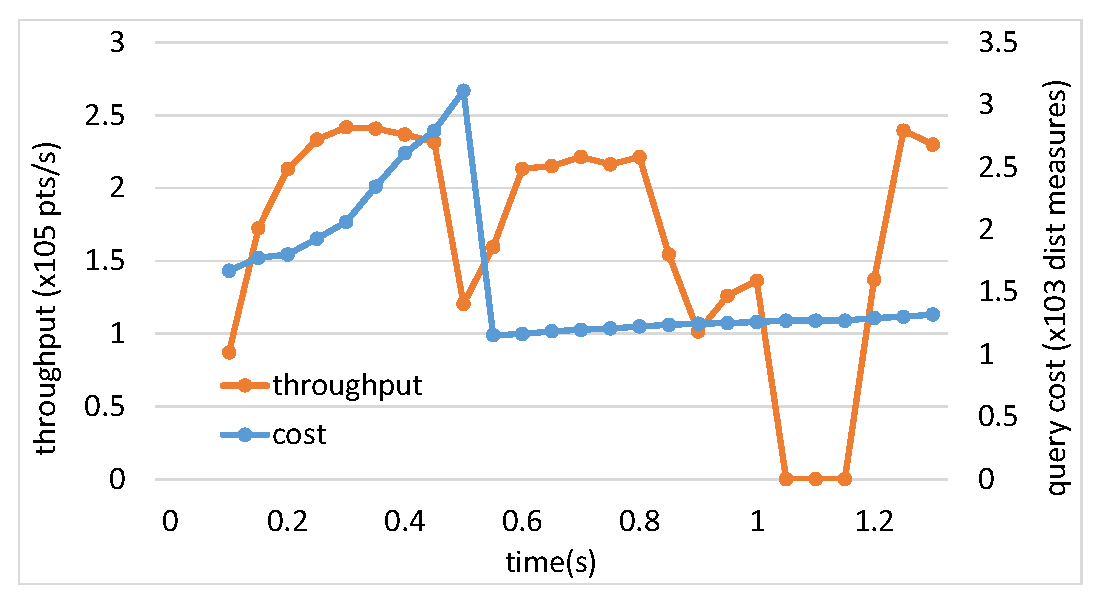
\includegraphics[width=2.6in]{fig/streaminsert.eps}}
    %\vspace{-0.1in}
    \caption{The processing throughput and query cost for a sequence of insertions.}
    %\vspace{-0.1in}
    \label{fig:streaminsert}
\end{figure}

The processing throughput and query cost results are shown in Figure \ref{fig:streaminsert}. We can see that the processing throughput is obviously reduced after each time window (0.5s and 1s) since many overloaded buckets will be split at that time. Note that, the throughput may also drop within a time window since some buckets might be seriously overloaded (i.e., the bucket size is larger than $(1+\epsilon_m)\cdot T_u$) and cannot wait for the time window to end. The query cost for a specific point will be continuously increased until some of its host buckets are split. From this figure, this happens after the first time window (0.5s). It is probably because one of the query's host buckets is split. In addition, the throughput should be affected by $\epsilon_m$ and $\epsilon_c$. We run experiments and see that the throughput is increased when increasing $\epsilon_m$. For $\epsilon_m=(0.2,0.4,0.6,0.8,1)$, the average throughput results is $(1.25,1.49,1.66,1.77,2.28)\times 10^5$ pts/s.

\begin{comment}
\subsection{Distributed All-Pairs Computation}
\label{sec:expr:allpair}

In Section \ref{sec:distributed}, we introduce a use case of distributed all-pairs computation, i.e., point density evaluation. We conduct experiments to show the benefit of our proposed multi-layered LSH structure in distributed computing. The experiment is performed in a large distributed cluster which contains 64 m1.medium Amazon EC2 instances. Each instance is equipped with 1 vCPU, 3.75GB memory, and 410GB disk. We utilize LSH and LayerLSH to partition the BigCross dataset and approximate the point densities by using Hadoop MapReduce. The MapReduce implementation involves two jobs. The first performs LSH partition and all-pairs computation locally. The second job aggregates the local results. The LSH parameters are set as $l=3, m=3$. The expected accuracy is set to 0.95 such that $w$ can be computed based on Equation (\ref{eq:prob2}), since the radius for evaluating point density is given. In LayerLSH, the bucket size limit is set as 10000 rather than being set according to precision rate, since this is not a $k$NN query application. In addition, similar sparse buckets are merged to further improve accuracy and to reduce number of partitions. The lower bound of bucket size is set as 1000. The number of reduce tasks is set as 256.

\begin{figure}[t]
%\vspace{-0.1in}
    \centerline{\includegraphics[angle=-90, width=2in]{fig/amazon_buckets.eps}}
    %\vspace{-0.05in}
    \caption{The distribution of bucket size in LSH and LayerLSH (BigCross).}
    %\vspace{-0.2in}
    \label{fig:amazon_buckets}
\end{figure}

By applying LSH and LayerLSH, the bucket size distributions are depicted in Figure \ref{fig:amazon_buckets}. The dense buckets are rehashed and the sparse buckets are merged in LayerLSH, so that the skewed buckets are balanced. As known, workload balance is crucial for distributed computing, which could bring significant performance gain especially in a very large scale distributed environment.

\begin{figure}[t]
%\vspace{-0.1in}
	\centerline{
	\subfloat[LSH]{\includegraphics[angle=-90, width=1.8in]{fig/lshruntime.eps}
    \label{fig:amazon:lsh}
    \vspace{-0.05in}}
    \hspace{-5mm}
    \subfloat[LayerLSH]{\includegraphics[angle=-90, width=1.8in]{fig/layerlshruntime.eps}
    \label{fig:amazon:layerlsh}
    \vspace{-0.05in}}
    }
    %\vspace{-0.05in}
	\caption{The runtime of point density evaluation using Hadoop (BigCross).}
	\label{fig:amazon}
%\vspace{-0.2in}
\end{figure}

The runtime of reduce tasks are shown in Figure \ref{fig:amazon}. Each color bar represents a reduce task, which performs local all-pairs computation. Each worker is assigned with multiple reduce tasks. The skewed distribution of bucket sizes leads to the skewed runtime of reduce tasks. We can see that the runtime of reduce tasks is seriously skewed when using LSH. While the runtime of reduce tasks in LayerLSH is more balanced. Accordingly, LSH-based point density evaluation requires much longer runtime than LayerLSH-based approach (20h58m2s vs. 1h36m38s). Since the rehashing strategy of LayerLSH does not reduce accuracy and the sparse buckets are merged, the accuracy is even higher by using LayerLSH\footnote{Because we cannot obtain the exact density values of all points in a reasonable time, we only show the sum of density values. In terms of point density's definition, the larger density should be more accurate.}.
\end{comment}



\section{Related Work}
\label{sec:related}

\Paragraph{LSH Variants} The LSH functions based on Euclidean space are proposed by Datar et at. \cite{datar}. Since then, a large number of LSH variants were proposed for improving accuracy and reducing I/O cost, including table-based LSH such as multi-probe LSH \cite{mplsh}, entropy LSH \cite{Panigrahy:2006:EBN:1109557.1109688}, C2LSH \cite{c2lsh}, and tree-based LSH such as LSB-tree \cite{lsb}, LSH Forest \cite{Bawa:2005:LFS:1060745.1060840}, SK-LSH \cite{sklsh}. Besides them, numerous excellent works are proposed in recent years. LazyLSH \cite{Zheng:2016:LAN:2882903.2882930} is able to answer approximate NN queries for multiple $l_p$ metrics. It uses a single base index to support the computations in multiple $l_p$ spaces. QALSH \cite{Huang:2015:QLH:2850469.2850470} introduces a novel concept of query-aware bucket partition which uses a given query as the anchor for bucket partition. This differs from the traditional LSH that partitions buckets ahead without any knowledge of the query distribution. SRS \cite{srs} requires only a single tiny index to answer approximate NN queries with theoretical guarantees.

%\Paragraph{LSH-based Applications} Researchers have leveraged the locality-preserving property of LSH to improve the performance in a wide range of applications. McConville et al. uses LSH to accelerate large scale centroid-based clustering \cite{lshcluster}. Liu et al. exploits LSH for distributed graph summarization \cite{graphsummarize}.

\Paragraph{Distributed LSH} A set of research works focus on design efficient distributed LSH indices for supporting large data sets. Zhang et al. utilize the locality preserving property of $z$-values and perform $z$-value based partition join in MapReduce to approximate the $k$NN joins \cite{Zhang:2012:EPK:2247596.2247602}. Haghani et al. propose mappings from the multi-dimensional LSH bucket space to the linearly ordered set of peers that jointly maintain the indexed data, so that buckets likely to hold similar data are stored on the same or neighboring peers in a P2P system \cite{Haghani:2009:DSS:1516360.1516446}. Bahmani et al. propose a distributed Entropy LSH implementation and prove that it exponentially decreases the network cost, while maintaining a good load balance between different machines \cite{distlsh}. PLSH \cite{Sundaram:2013:SSS:2556549.2556574} is a parallel LSH that supports high-throughput streaming of new data, which exploits an insert-optimized hash table structure and efficient data expiration algorithm for streaming data.

\Paragraph{Data Sensitive Hashing} As discussed in Section \ref{sec:intro}, the recently proposed data sensitive hashing, e.g., DSH \cite{Gao:2014:DDS:2588555.2588565} and selective hashing \cite{Gao:2015:SHC:2783258.2783284}, are the first works that leverage data distributions. However, rather than learning the optimal hash functions from the skewed data, our approach relies on postprocessing and leverages the density of hash values to reorganize the existing structures. It is orthogonal to the data sensitive hashing. As presented in Section \ref{sec:extension:dsh} and Section \ref{sec:expr:dsh}, we can rebuild DSH index as a postprocessing step to further improve performance. HashFile \cite{Zhang:2011:HEI:2004686.2005629} also proposes to recursively partition the dense buckets. However, we use a multi-layered structure to organize the points as a general strategy that also benefits the tree-like LSH indices, which differs from it. The most relevant work is the recently proposed neighbor-sensitive hashing (NSH) \cite{Park:2015:NH:2850583.2850589}. The NSH and our work share the same intuition that the limited hash bits should be used to better distinguish nearby items instead of capturing the distances among far apart items. However, NSH aims to devise a new hashing mechanism to achieve this goal, while we propose to reconstruct the existing LSH index structures as a postprocessing step, which is different from NSH.



\section{Conclusion}
\label{sec:conclusion}

In this paper, we present the layered version of LSH variants by exploring the density of hash values. The dense buckets are rehashed and the sparse buckets are merged in order to make the hashing more targeted in terms of data distribution. Based on this idea, we rebuild the basic LSH, LSB, and DSH, and propose LayerLSH, LayerLSB, and LayerDSH for illustration. We also discuss the possibilities of rebuilding other LSH variants and demonstrate the benefit in distributed computing. The experimental studies have shown their effectiveness and efficiency. Specifically, LayerLSH can reach the same search quality as LSH with only 5\%-20\% query cost.


\bibliographystyle{abbrv}
\bibliography{./references}

%\input{Appendix}

\end{document}


